\documentclass[a4paper,12pt,twoside]{article}
\usepackage{amsmath}
\usepackage{amssymb}
\usepackage{bm}
\usepackage{booktabs}
\usepackage[small,bf]{caption}
\usepackage{comment}
\usepackage{cuted}
\usepackage[shortlabels]{enumitem}
\usepackage{fancyhdr}
\usepackage{fancybox}
\usepackage{float}
\usepackage[T1]{fontenc}
\usepackage[a4paper,left=1in,right=1in,top=0.25in,bottom=1in,
    headheight=76.33466pt,
    headsep=\dimexpr1in-62.33466pt\relax,
    includehead
]{geometry}
\usepackage{graphicx}
\usepackage{hyperref}
\usepackage[utf8]{inputenc}
% \usepackage{lipsum}
\usepackage{listings}
\usepackage{minted}
\usemintedstyle{emacs}
\usepackage{multirow}
\usepackage{parskip}
\usepackage{ragged2e}
\usepackage{setspace}
\usepackage{soul}
% \onehalfspacing
\usepackage{subcaption}
% \usepackage[subrefformat=parens,labelformat=parens]{subfig}
\usepackage{tabularx}
% \usepackage{titling}
\usepackage{xurl}
\usepackage{biblatex}
\addbibresource{Lab3.bib}
\usepackage{background}
\backgroundsetup{contents=
\includegraphics{waterprint.jpg}, scale=0.8, opacity=0.1}
\pagestyle{fancy}
\fancyhf{}
\fancyhead[LE,RO]{}
\fancyhead[CE,CO]{
\includegraphics[width=0.7\textwidth]{JILogo.png}}
\fancyhead[RE,LO]{}
\fancyfoot[CE,CO]{\leftmark}
\fancyfoot[CE,CO]{\thepage}
\lfoot{\textit{ECE4810J \textbf{SoC Design} | Fall 2022}}
\renewcommand{\headrulewidth}{1pt}
\renewcommand{\footrulewidth}{1pt}
\definecolor{caption2color}{HTML}{2e5395}
\hypersetup{
    colorlinks=true,
    linkcolor=blue,
    filecolor=magenta,      
    urlcolor=cyan,
    pdfpagemode=FullScreen,
}
\definecolor{codegreen}{rgb}{0,0.6,0}
\definecolor{codegray}{rgb}{0.5,0.5,0.5}
\definecolor{codepurple}{rgb}{0.58,0,0.82}
\definecolor{backcolour}{rgb}{0.95,0.95,0.92}

\lstdefinestyle{mystyle}{
    backgroundcolor=\color{backcolour},   
    commentstyle=\color{codegreen},
    keywordstyle=\color{magenta},
    numberstyle=\tiny\color{codegray},
    stringstyle=\color{codepurple},
    basicstyle=\ttfamily\footnotesize,
    breakatwhitespace=false,         
    breaklines=true,                 
    captionpos=b,                    
    keepspaces=true,                 
    numbers=left,                    
    numbersep=5pt,                  
    showspaces=false,                
    showstringspaces=false,
    showtabs=false,                  
    tabsize=2
}

\lstset{style=mystyle}

\author{Xinfei Guo, Yihua Liu}
\title{ECE4810J FA2021\\ \small Lab \#1}
\date{September 28, 2022}

\begin{document}
% \maketitle
\thispagestyle{fancy}

\begin{center}
    \vspace*{0pt}
    \Large{\textbf{ECE4810J SoC Design}}\\
    \vspace*{2pt}
    \large{Fall 2022}\\
    \vspace*{10pt}
    \Large{\textcolor{caption2color}{Lab \#3 PYNQ Overlays \& Optimizing HLS Performance through Pipelining}}\\
    \normalsize{\hl{Due: 11:59pm Oct. 23rd, 2022}}
    \rule[-5pt]{.97\linewidth}{0.05em}
\end{center}

\textbf{Logistics:}
\begin{itemize}
    \item This lab is a team exercise.
    \item Please use the discussion board on Piazza for Q\&A.
    \item All reports and code (if available) MUST be submitted to the assignment of Canvas.
    \item Internet usage is allowed and encouraged.
    \item No late submission is allowed for this lab.
\end{itemize}
\newpage
\tableofcontents
\newpage
\section{Overview}
In this lab, you will learn about PYNQ overlays and exercise the HLS flow on Zynq using Vitis HLS. The goals of this lab are to:
\begin{itemize}
    \item Load overlay, use overlay and create overlays
    \item Understand the effect of the INLINE directive
    \item Improve performance using PIPELINE directive
    \item Distinguish between DATAFLOW directive and Configuration Command functionality
\end{itemize}

% \section{Debug HLS}
% \begin{enumerate}
%     \item Create a Vitis HLS project matrixmul with top function \texttt{matrixmul}. Add matrixmul.h and matrixmul.cpp as the Source, and ad matrixmul\_test.cpp s the Test Bench.
%     \item Run C Simulation, check the Launch Debugger option. The application will be compiled with \texttt{–g} option to include the debugging information, the compiled application will be invoked, and the debug perspective will be opened automatically. The Debug perspective will show \texttt{argc} and \texttt{argv} variables defined in the Variables view and thread created and the program suspended at the main() function entry point in the *Debug* view.
%     \begin{figure}[H]
%         \centering
%         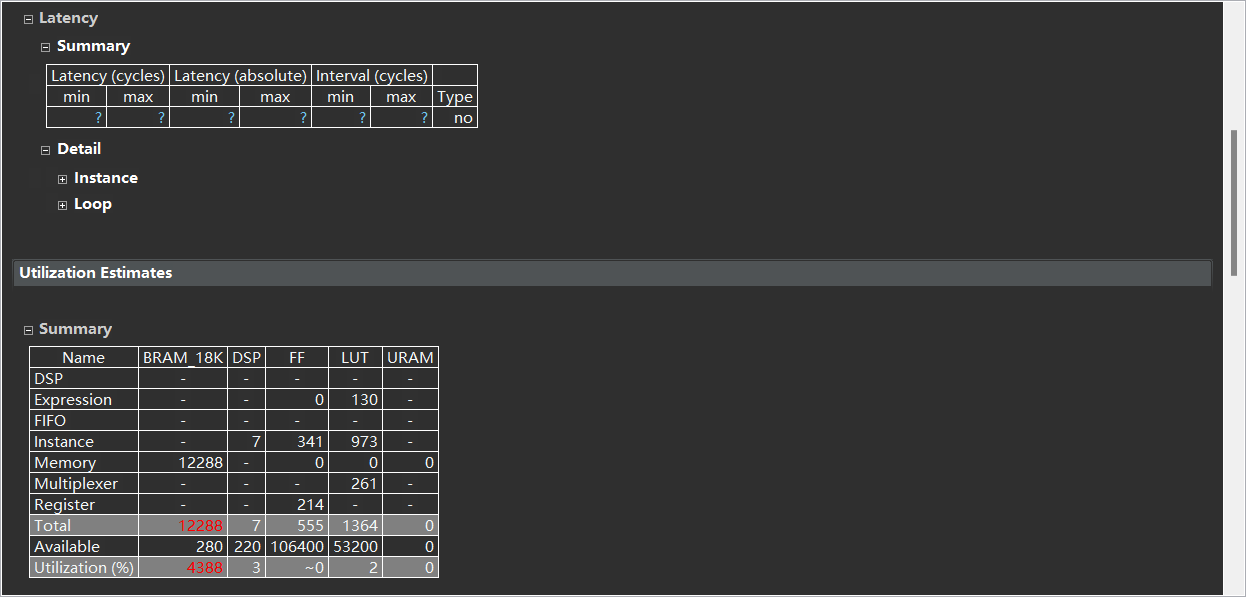
\includegraphics[width=\textwidth]{images/1.png}
%         \caption{A Debug perspective.}
%     \end{figure}
%     \item Scroll down the Test Bench file, double-click in the blue margin at line 105:
%     \begin{minted}[breaklines,linenos,escapeinside=||]{c++}
%     cout << "{" << endl;|\setcounter{FancyVerbLine}{105}|
%     \end{minted}
%     The breakpoint is marked with a blue circle. Similarly, set a breakpoint at line 101.
%     \begin{minted}[breaklines,linenos,escapeinside=||]{c++}
%     matrixmul(in_mat_a, in_mat_b, hw_result);|\setcounter{FancyVerbLine}{101}|
%     \end{minted}
%     \item In the top bar under the menu bar, click the "Step Over" button or press F6 several times, observe the execution progress, and observe the variable values updating, as well as the computed software result.
%     \item Click the "Resume" button or press F8 to complete the software computation and stop at line 101.
%     \item Click on the Step Into button or press F5 to traverse into the \texttt{matrixmul} module, the one that we will synthesize, and observe that the execution is paused on line 75 of the module.
%     \item Using the Step Over several times, observe the computed results. Once satisfied, you can use the Step Return button or press F7 to return from the function.
%     \item The program execution will suspend at line 105 as we had set a breakpoint. Observe the software and hardware (function) computed results in the Variables view.
% \end{enumerate}

\section{Optimize Performance through Pipelining}\label{S2}
\subsection{YUV model}
The YUV model defines one luminance component (Y), meaning physical linear-space brightness, and two chrominance components called U (blue projection) and V (red projection), respectively. It can be used to convert to and from the RGB model, and with different color spaces. The closely related Y'UV model uses the luma component (Y') – nonlinear perceptual brightness, with the prime symbols (') denoting gamma correction \cite{enwiki:1114229318}. Today, the term YUV is commonly used in the computer industry to describe colorspaces that are encoded using YCbCr, used for digital encoding of color information suited for video and image compression and transmission formats like MPEG \& JPEG.
\begin{figure}[H]
    \centering
    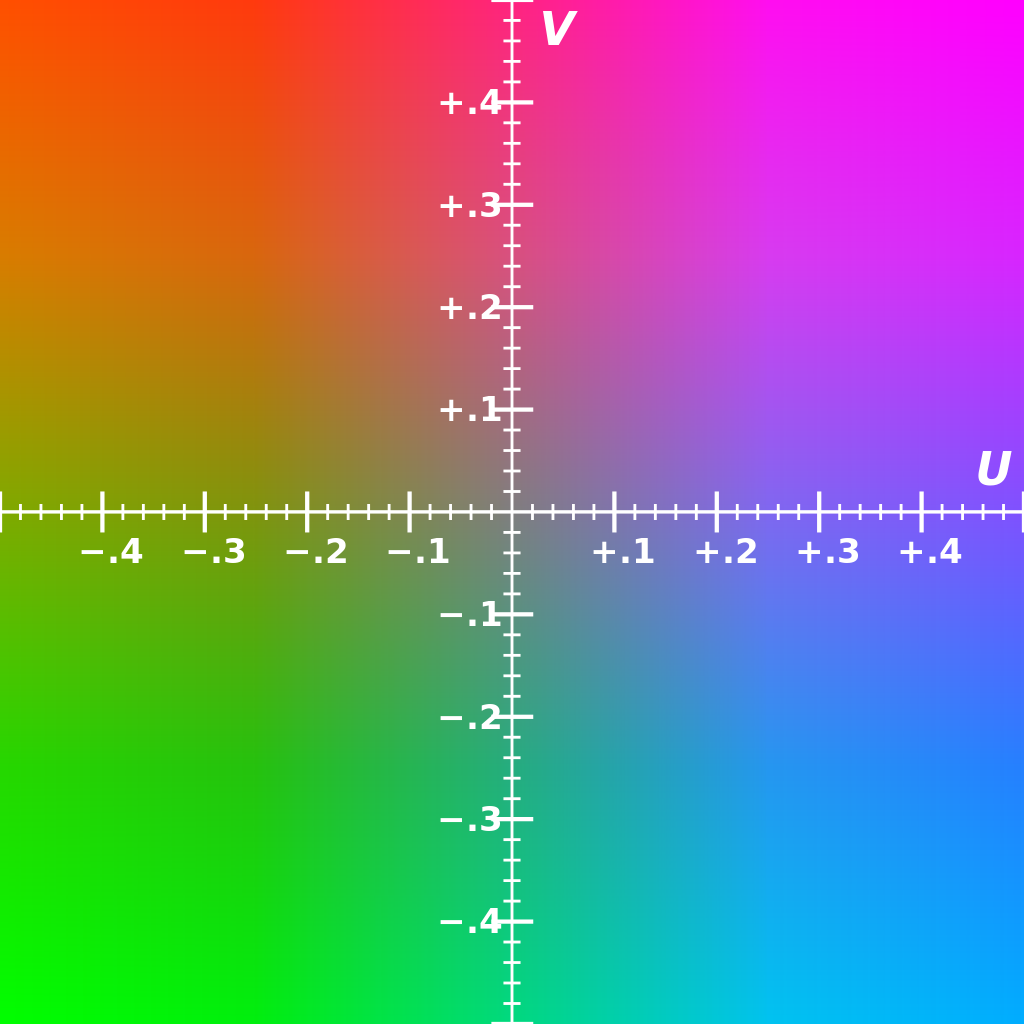
\includegraphics[width=0.6\textwidth]{images/10.png}
    \caption{Example of U-V color plane, $Y' = 0.5$, represented within RGB color gamut \cite{yuvsvg}.}
\end{figure}
Y'UV files can be encoded in 12, 16, or 24 bits per pixel. The common formats are:
\begin{table}[H]
    \centering
    \begin{tabular}{|c|c|c|c|c|}
        \hline
        \multirow{2}{*}{Name} & \multirow{2}{*}{Size} & \multicolumn{3}{c|}{Ratio}\\
        \cline{3-5}
        && A:B:C & Horizontal & Vertical\\
        \hline
        Y'UV444/YUV444 & 3 bytes per pixel & 4:4:4 & Full & Full \\
        \hline
        Y'UV422/YUV422 & 4 bytes per 2 pixels & 4:2:2 & 2:1 & Full \\
        \hline
        Y'UV420p/YUV420 & 6 bytes per 4 pixels, reordered & 4:2:0 & 2:1 & 2:1 \\
        \hline
        YUV411 & 6 bytes per 4 pixels & 4:1:1 & 4:1 & Full \\
        \hline
    \end{tabular}
    \caption{YUV A:B:C (or 4:x:x) based on the NTSC (National Television System Committee) standard, a standard for analog television broadcasts.}
\end{table}
RGB888 is R-8bit, G-8bit, B-8bit, i.e., RGB24.

For the conversion from RGB to Y'UV:
\begin{align}
  Y' &=  0.299 R + 0.587 G + 0.114 B \\
  U  &= -0.147 R - 0.289 G + 0.436 B \\
  V  &=  0.615 R - 0.515 G - 0.100 B
\end{align}
On older, non-SIMD architectures, floating point arithmetic is much slower than using fixed-point arithmetic, so most digital implementations of RGB \textrightarrow Y'UV used integer math, in particular fixed-point approximations. Approximation means that the precision of the used numbers (input data, output data, and constant values) is limited, and thus a precision loss of typically about the last binary digit is accepted by whoever makes use of that option in typically a trade-off to improved computation speeds \cite{enwiki:1114229318}. Y' values are conventionally shifted and scaled to the range [16, 235] (referred to as studio swing or "TV levels") rather than using the full range of [0, 255] (referred to as full swing or "PC levels"). This practice was standardized in SMPTE-125M in order to accommodate signal overshoots ("ringing") due to filtering. The value 235 accommodates a maximal black-to-white overshoot of $255 - 235 = 20$, or $20 / (235 - 16) = 9.1\%$, which is slightly larger than the theoretical maximal overshoot (Gibbs phenomenon) of about 8.9\% of the maximal step. The toe-room is smaller, allowing only 16 / 219 = 7.3\% overshoot, which is less than the theoretical maximal overshoot of 8.9\%. This is why 16 is added to Y' and why the Y' coefficients in the basic transform sum to 220 instead of 255 \cite{yuvjack}. U and V values, which may be positive or negative, are summed with 128 to make them always positive, giving a studio range of 16–240 for U and V. (These ranges are important in video editing and production since using the wrong range will result either in an image with "clipped" blacks and whites, or a low-contrast image.)

For getting the traditional "studio-swing" 8-bit representation of YCbCr for SDTV/BT.601 the following operations can be used:
\begin{enumerate}
    \item Basic transform from 8-bit RGB to 16-bit values (Y': unsigned, Cb/Cr: signed, matrix values got rounded so that the later-on desired Y' range of [16..235] and Cb/Cr range of [16..240] is reached):
    \begin{equation}
        \begin{bmatrix}
        Y'\\
        Cb\\
        Cr
        \end{bmatrix}=
        \begin{bmatrix}
        66&129&25\\
        -38&-74&112
        \\112&-94&-18
        \end{bmatrix}
        \begin{bmatrix}
        R\\
        G\\
        B
        \end{bmatrix}.
    \end{equation}
    \item Scale down to 8 bits with rounding ("+128") (Y': unsigned, Cb/Cr: signed):
    \begin{equation}
        \begin{aligned}
            Y_{t}'&=(Y'+128)\gg 8,\\
            Cb_{t}&=(U+128)\gg 8,\\
            Cr_{t}&=(V+128)\gg 8.
        \end{aligned}
    \end{equation}
    \item Add an offset to the values to eliminate any negative values (all results are 8-bit unsigned):
    \begin{equation}
        \begin{aligned}
            Y_{u}'&=Y_{t}'+16,\\
            Cb_{u}&=Cb_{t}+128,\\
            Cr_{u}&=Cr_{t}+128.
        \end{aligned}
    \end{equation}

\end{enumerate}

An alternative formulation provided by Microsoft DirectDraw (a component of DirectX API) is \cite{directdraw}:
\begin{align}
Y' &= ( (  66 R + 129 G +  25 B + 128) \gg 8) +  16 \\
U  &= ( ( -38 R -  74 G + 112 B + 128) \gg 8) + 128 \\
V  &= ( ( 112 R -  94 G -  18 B + 128) \gg 8) + 128
\end{align}
These formulas produce 8-bit results using coefficients that require no more than 8 bits of (unsigned) precision. Intermediate results require up to 16 bits of precision. For the conversion from Y'UV to RGB, using the coefficients $c$, $d$, and $e$, and noting that {$[]_{0}^{255}$} denotes clamping a value to the 8-bit range of 0 to 255, the following formulae provide the conversion from Y'UV to RGB (NTSC version):
\begin{align}
  c &= Y' - 16 \\
  d &= U - 128 \\
  e &= V - 128
\end{align}
\begin{align}
  R &= [( 298 c                + 409 e + 128) \gg 8]_0^{255} \\
  G &= [( 298 c - 100 d - 208 e + 128) \gg 8]_0^{255} \\
  B &= [( 298 c + 516 d                + 128) \gg 8]_0^{255}
\end{align}
In Microsoft documentation, the clamping is also denoted as a function \texttt{clip()}:
\begin{align}
R &= \mathrm{clip}(( 298  c          + 409  e + 128) \gg 8)\\
G &= \mathrm{clip}(( 298  c - 100  d - 208  e + 128) \gg 8)\\
B &= \mathrm{clip}(( 298  c + 516  d          + 128) \gg 8)
\end{align}
These formulas use some coefficients that require more than 8 bits of precision to produce each 8-bit result, and intermediate results require more than 16 bits of precision. Given the knowledge, you can fill your lab3\_starter/yuv\_filter.c now. Note that the macro \texttt{CLIP} has already been well defined in lab3\_starter/yuv\_filter.h.

Besides, you also need to prepare your input data \texttt{lab3\_starter/yuv\_filter/input.dat} from the standard test image \texttt{lab3\_starter/lena\_std.tif} \cite{lenaimg}. One possible way is to use MATLAB:
\begin{minted}{matlab}
lena_std = imread('lena_std.tif');
std_perm = permute(lena_std, [2 3 1]);
dlmwrite('input.dat', std_perm, 'delimiter', '\n')
\end{minted}
The matrix is permuted in this way because we want the output dimension order conforms to the dimension order of the function \texttt{image\_read} in \texttt{lab3\_starter/image\_aux.c}. \textbf{Remember to run \texttt{make clean} before \texttt{make} if you \texttt{make} multiple times.}

After you generate the \texttt{output.dat}, convert it back to a TIF file \texttt{lena\_rec.tif} (other image formats are also OK). The sample MATLAB script is
\begin{minted}{matlab}
output = dlmread('lab3/output.dat');
img_rec = reshape(output, 3, 512, 512);
img_rec_perm = permute(img_rec, [3 2 1]);
imwrite(uint8(img_rec_perm), 'lena_rec.tif');
\end{minted}

\subsection{Create a Vitis HLS project from command line}
\begin{enumerate}
    \item Open Vitis HLS 2022.1 Command Prompt.
    \item Change directory to your lab directory. A self-checking program \texttt{yuv\_filter\_test.c} is provided. Using that, we can validate the design. A Makefile is also provided. Using the Makefile, the necessary source files can be compiled, and the compiled program can be executed. You can examine the contents of these files and the project directory.
    \item Run \texttt{make} to compile and execute the program. If it fails, read Appendix \ref{AMake}. You should see the output
    \begin{minted}[breaklines,breakanywhere]{text}
gcc -ggdb -w -I/f/Xilinx/Vitis_HLS/2022.1/include   -c -o yuv_filter.o yuv_filter.c
gcc -ggdb -w -I/f/Xilinx/Vitis_HLS/2022.1/include   -c -o yuv_filter_test.o yuv_filter_test.c
gcc -ggdb -w -I/f/Xilinx/Vitis_HLS/2022.1/include   -c -o image_aux.o image_aux.c
gcc -lm   yuv_filter.o yuv_filter_test.o image_aux.o   -o yuv_filter
./yuv_filter
Test passed!

    \end{minted}
    Note that the source files (yuv\_filter.c, yuv\_filter\_test.c, and image\_aux.c) were compiled, then the yuv\_filter executable program was created, and then it was executed. Only Verilog RTL and VHDL RTL are generated. If you also want to generate SystemC RTL, change Line 13 of Makefile to:
    \begin{minted}[breaklines,breakanywhere]{makefile}
USE_SYSTEMC 				= true
    \end{minted}
    A Vitis HLS Tcl script file pynq\_yuv\_filter.tcl is provided and can be used to create a Vitis HLS project.
    \item Run \texttt{vitis\_hls –f pynq\_yuv\_filter.tcl} in the Vitis HLS Command Prompt window to create the project targeting xc7z020clg400-1 part. The project will be created, and the vitis\_hls.log file will be generated. You can see the output in vitis\_hls.log.
    \item Open the created project in GUI mode from the Vitis HLS Command Prompt window by running \texttt{vitis\_hls -p yuv\_filter.prj}. The Vitis HLS will open in GUI mode, and the project will be opened. Note that different old Vivado HLS, new Vitis HLS automatically enables loop pipelining, so if you keep default settings, you will see the following in vitis\_hls.log and yuv\_filter.prj/solution1/solution1.log:
    \begin{minted}[breaklines,breakanywhere]{text}
INFO: [XFORM 203-510] Pipelining loop 'RGB2YUV_LOOP_Y' (yuv_filter.c:34) in function 'yuv_filter' automatically.
INFO: [XFORM 203-510] Pipelining loop 'YUV_SCALE_LOOP_Y' (yuv_filter.c:118) in function 'yuv_filter' automatically.
INFO: [XFORM 203-510] Pipelining loop 'YUV2RGB_LOOP_Y' (yuv_filter.c:72) in function 'yuv_filter' automatically.
    \end{minted}
    To prevent this, open tab yuv\_filter.c. Menu Window->Show View->Directive, open Directive tab, for each of `rgb2yuv`, `yuv2rgb`, and `yuv\_scale`, right-click it, Insert Directive... In the pop-up window Vitis HLS Directive Editor, Directive: PIPELINE, check Options: off (optional). After doing this, you will see a new directive: HLS PIPELINE off. Run C Synthesis->Active Solution again.
\end{enumerate}
\subsection{Analyze the created project and results}
\begin{enumerate}
    \item In Vitis HLS GUI, expand the source folder in the \textit{Explorer} view and double click yuv\_filter.c to view the content. The design is implemented in 3 functions: rgb2yuv, yuv\_scale, and yuv2rgb. Each of these filter functions iterates over the entire source image (which has maximum dimensions specified in image\_aux.h), requiring a single source pixel to produce a pixel in the resulting image. The scale function simply applies individual scale factors, supplied as top-level arguments to the Y’UV components. Notice that most of the variables are user-defined (typedef) and aggregate (e.g. structure, array) types. A viable workaround is conditionally compiled into the code, leveraging the \texttt{\_\_SYNTHESIS\_\_} macro. Vitis HLS automatically defines the \texttt{\_\_SYNTHESIS\_\_} macro when reading any code. This ensures the original \texttt{malloc()} code is used outside of synthesis, but Vitis HLS will use the workaround when synthesizing.
    \item Expand the solution1 > syn > report folder in the \textit{Explorer} view and double-click yuv\_filter\_csynh.rpt entry to open the synthesis report. Each of the loops in this design has variable bounds – the width and height are defined by members of input type image\_t. When variable bounds are present on loops, the total latency of the loops cannot be determined: this impacts the ability to perform analysis using reports. Hence, “?” is reported for various latencies.
    \begin{figure}[H]
        \centering
        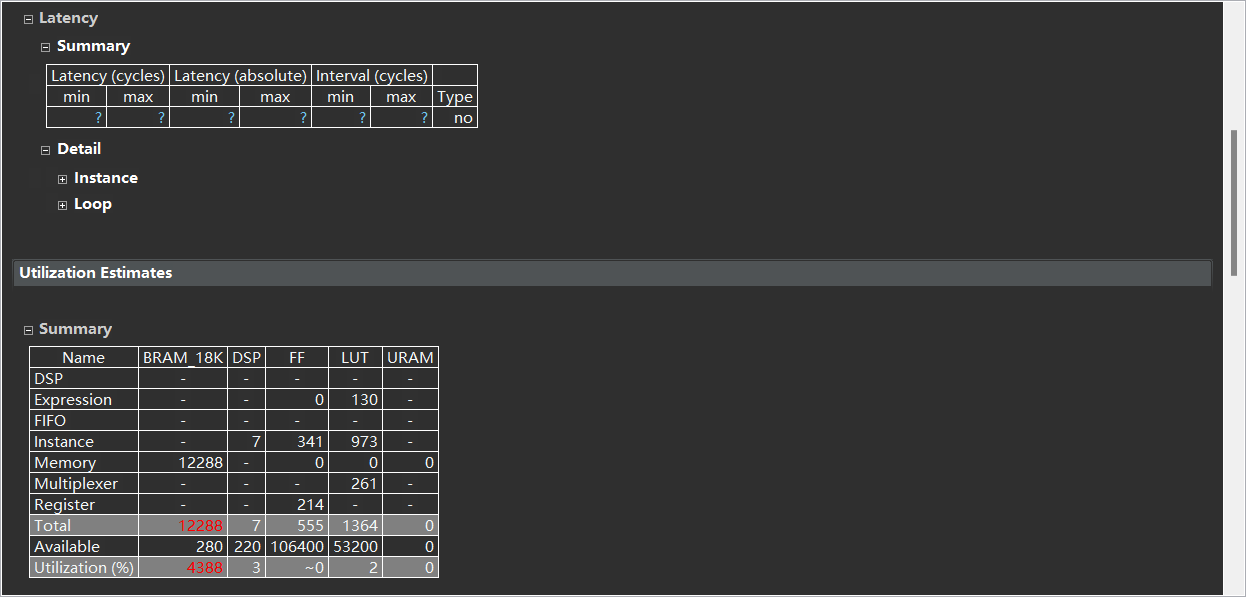
\includegraphics[width=\textwidth]{images/1.png}
        \caption{Latency computation.}
    \end{figure}
    You can scroll down to the bottom of the report and click the "Export Dialog" to export the report to an HTML format file. Then, you can convert HTML to PDF.
\end{enumerate}
\subsection{Apply \texttt{TRIPCOUNT} pragma}\label{S23}
Open the source file and uncomment pragma lines, re-synthesize, and observe the resources used as well as estimated latencies. Answer the questions listed in the detailed section of this step.
\begin{enumerate}
    \item To assist in providing loop-latency estimates, Vitis HLS provides a \texttt{TRIPCOUNT} directive, which allows limits on the variables' bounds to be specified by the user. In this design, such directives have been embedded in the source code, in the form of \texttt{\#pragma} statements.
    \item Uncomment the \texttt{\#pragma} lines (50, 53, 90, 93, 130, 133) to define the loop bounds and save the file.
    \item Synthesize the design by selecting Solution > Run C Synthesis > Active Solution. View the synthesis report when the process is completed.
    % \textbf{Question 1}\\
    % Answer the following question pertaining to yuv\_filter function.\\
    % Estimated clock period:\\  % 6.651 ns
    % Worst case latency:\\
    % Number of DSP48E used:\\
    % Number of BRAMs used:\\
    % Number of FFs used:\\
    % Number of LUTs used:
    \item Scroll the \textit{Console} window and note that the yuv\_scale function is automatically inlined into the yuv\_filter function.
    \begin{figure}[H]
        \centering
        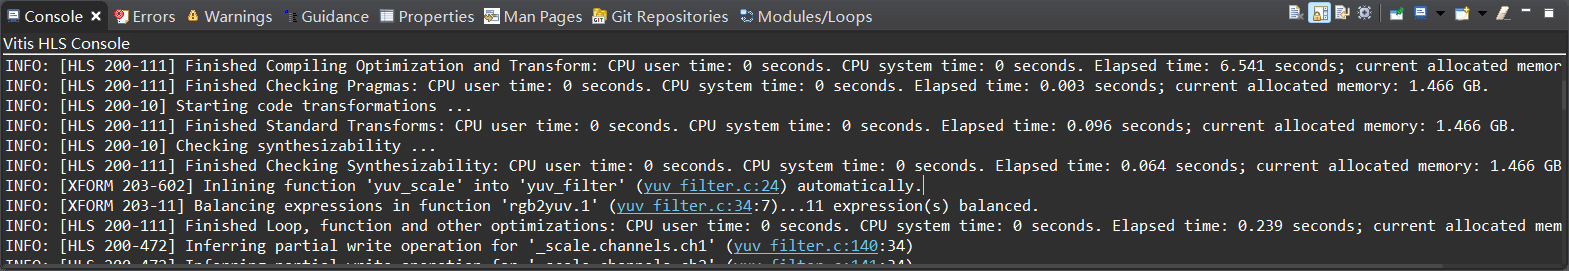
\includegraphics[width=\textwidth]{images/2.png}
        \caption{Vitis HLS automatically inlining function.}
    \end{figure}
    \item Observe that there are three entries – rgb2yuv.rpt, yuv\_filter.rpt, and yuv2rgb.rpt under the syn report folder in the Explorer view. There is no entry for yuv\_scale.rpt since the function was inlined into the yuv\_filter function. You can access the lower-level module’s report by either traversing down in the top-level report under components (under Utilization Estimates > Details > Component) or from the reports container in the project explorer.
    \item Expand the Summary of loop latency and note the latency and trip count numbers for the yuv\_scale function. Note that the YUV\_SCALE\_LOOP\_Y loop latency is 4x the specified TRIPCOUNT, implying that four cycles are used for each iteration of the loop.
    \begin{figure}[H]
        \centering
        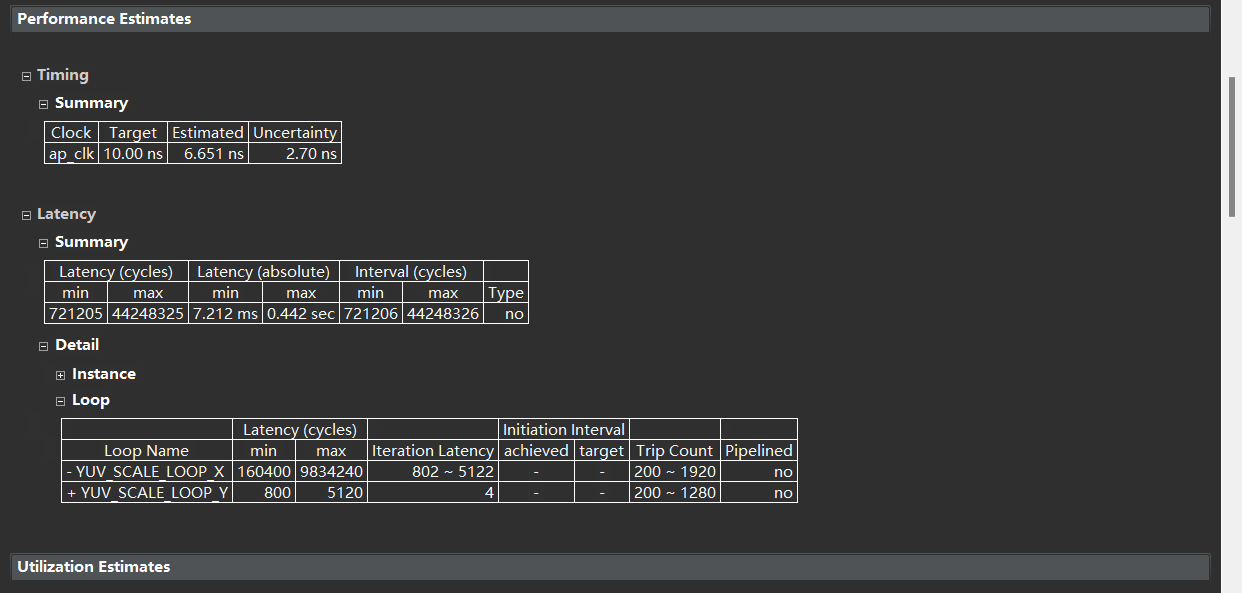
\includegraphics[width=\textwidth]{images/3.png}
        \caption{Loop latency.}
    \end{figure}
    \item You can verify this by opening an analysis perspective view in the Solution menu->Open Schedule Viewer, expanding the YUV\_SCALE\_LOOP\_X entry, and then expanding the YUV\_SCALE\_LOOP\_Y entry.
    \begin{figure}[H]
        \centering
        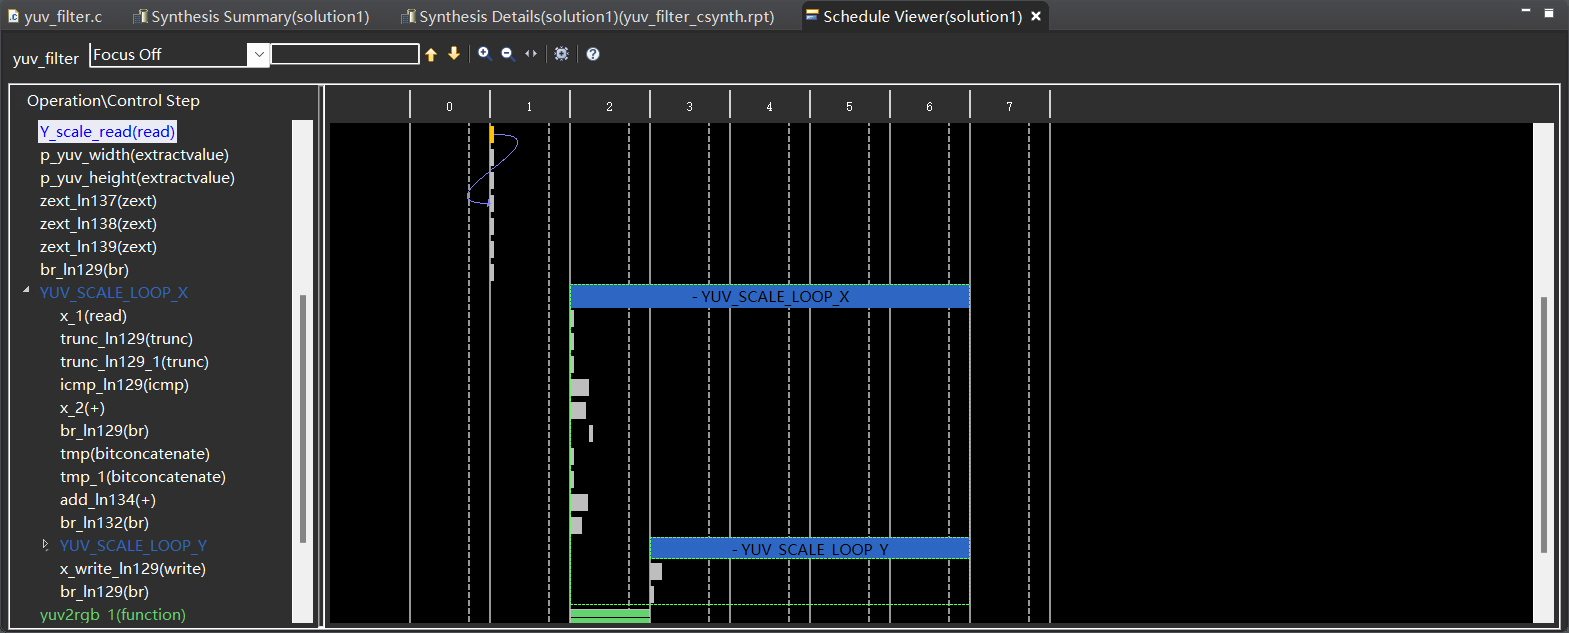
\includegraphics[width=\textwidth]{images/4.png}
        \caption{Design analysis view of the YUV\_SCALE\_LOOP\_Y loop.}
    \end{figure}
    \item In the Synthesis Details, expand Detail > Instance section of the Utilization Estimates and click on the grp\_rgb2yuv\_fu\_251 (rgb2yuv\_1) entry to open the report Synthesis Details(solution1)(rgb2yuv\_1\_csynth.rpt).
    \item Similarly, click on the grp\_yuv2rgb\_fu\_271 entry to open the report Synthesis Details(solution1)(yuv2rgb\_1\_csynth.rpt).
    \item Report the following metrics of yuv\_filter, rgb2yuv, and yuv2rgb functions:
    \begin{enumerate}
        \item Estimated clock period
        \item Worst case latency
        \item Number of DSP48E used
        \item Number of BRAMs used
        \item Number of FFs used
        \item Number of LUTs used
    \end{enumerate}
\end{enumerate}
\subsection{Turn off \texttt{INLINE} and apply \texttt{PIPELINE} directive}\label{S24}
Create a new solution by copying the previous solution settings. Prevent the automatic \texttt{INLINE} and apply \texttt{PIPELINE} directive. Generate the solution and understand the output.
\begin{enumerate}
    \item Select Project menu > New Solution...; in the pop-up Solution Wizard, check "Copy directives and constraints from solution:" and select solution1 in the Options frame.
    \item Make sure that the yuv\_filter.c source is opened and visible, and click on the \textbf{Directive} tab.
    \item Select function yuv\_scale in the directives pane, right-click on it and select Insert Directive...
    \item Click on the drop-down button of the Directive field in the pop-up Vitis HLS Directive Editor showing up listing various directives. Select INLINE directive.
    \item Click on the off (optional) option to turn off the automatic inlining. Make sure that the Directive File is selected as the destination. Click OK. When an object (function or loop) is pipelined, all the loops below it, down through the hierarchy, will be automatically unrolled. In order for a loop to be unrolled, it must have fixed bounds: all the loops in this design have variable bounds, defined by an input argument variable to the top-level function. Note that the \texttt{TRIPCOUNT} directive on the loops only influences reporting, it does not set bounds for synthesis. Neither the top-level function nor any of the sub-functions are pipelined in this example. The pipeline directive must be applied to the inner-most loop in each function – the innermost loops have no variable-bounded loops inside which are required to be unrolled, and the outer loop will simply keep the inner loop fed with data.
    \item Expand the yuv\_scale in the Directives tab, right click on \texttt{HLS PIPELINE off} directive; select "Remove Directive". Similarly, remove the \texttt{HLS PIPELINE off} directive of rgb2yuv and yuv2rgb. % right-click on YUV\_SCALE\_LOOP\_Y object and select insert directives …, and select PIPELINE as the directive. Leave II (Initiation Interval) blank as Vitis HLS will try for an II=1, one new input every clock cycle. Click OK.
    \item Run C Synthesis for solution2. You can observe the output:
    \begin{minted}[breaklines,breakanywhere]{text}
INFO: [SCHED 204-61] Pipelining loop 'RGB2YUV_LOOP_X_RGB2YUV_LOOP_Y'.
INFO: [HLS 200-1470] Pipelining result : Target II = NA, Final II = 1, Depth = 9, loop 'RGB2YUV_LOOP_X_RGB2YUV_LOOP_Y'
INFO: [SCHED 204-61] Pipelining loop 'YUV_SCALE_LOOP_X_YUV_SCALE_LOOP_Y'.
INFO: [HLS 200-1470] Pipelining result : Target II = NA, Final II = 1, Depth = 7, loop 'YUV_SCALE_LOOP_X_YUV_SCALE_LOOP_Y'
INFO: [SCHED 204-61] Pipelining loop 'YUV2RGB_LOOP_X_YUV2RGB_LOOP_Y'.
INFO: [HLS 200-1470] Pipelining result : Target II = NA, Final II = 1, Depth = 11, loop 'YUV2RGB_LOOP_X_YUV2RGB_LOOP_Y'
    \end{minted}
    \item When the synthesis is completed, select Project > Compare Reports… to compare the two solutions. Select Solution1 and Solution2 from the Available Reports in the Solution Selection Dialog, and click on the Add>> button.
    \item Observe the latency reduced in the Vitis HLS Report Comparison.
    \begin{figure}[H]
        \centering
        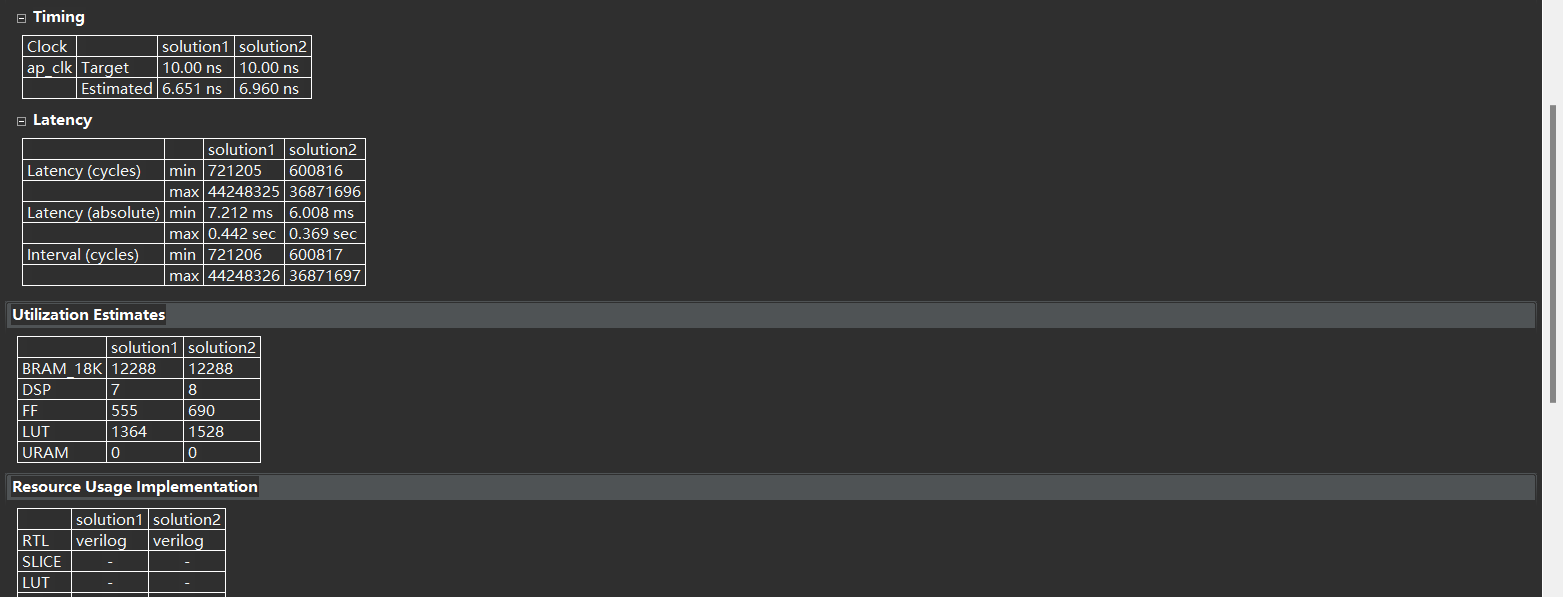
\includegraphics[width=0.9\textwidth]{images/5.png}
        \caption{Performance comparison after pipelining yuv\_scale only.}
    \end{figure}
    \begin{figure}[H]
        \centering
        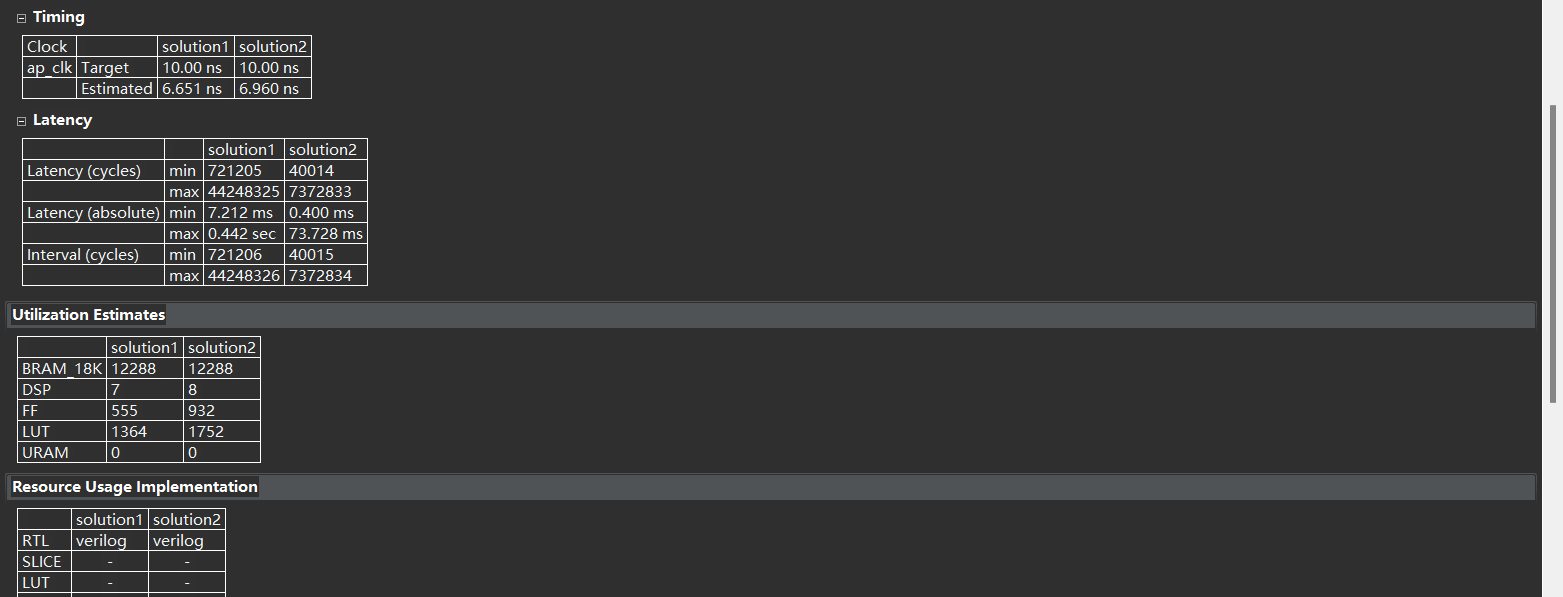
\includegraphics[width=0.9\textwidth]{images/6.png}
        \caption{Performance comparison after pipelining.}
    \end{figure}
    In Solution1, the total loop latency of the inner-most loop was loop\_body\_latency x loop iteration count, whereas in Solution2 the new total loop latency of the inner-most loop is loop\_body\_latency + loop iteration count. Scroll down in the comparison report to view the resource utilization. Observe that the FFs, LUTs, and DSP48E utilization increased, whereas BRAM remained the same. Take a screenshot of the Performance Estimates and Utilization Estimates of the Vitis HLS Report Comparison.
\end{enumerate}
\subsection{Apply \texttt{DATAFLOW} Directive and Configuration Command}\label{S25}
Create a new solution by copying the previous solution (Solution2) settings. Apply \texttt{DATAFLOW} directive. Generate the solution and understand the output.
\begin{enumerate}
    \item Create a new solution by copying the previous solution (Solution2) settings.
    \item Close all inactive solution windows by selecting Project menu > Close Inactive Solution Tabs.
    \item Make sure that the yuv\_filter.c source is opened in the information pane and select the \textit{Directive} tab.
    \item Insert the \texttt{DATAFLOW} directive for yuv\_filter function.
    \item Run C Synthesis. When the synthesis is completed, the synthesis report is automatically opened. Open the Synthesis Details(solution3)(yuv\_filter\_csynth.rpt) report from Explorer.
    \item Observe additional information, Dataflow Type, in the \textit{Performance Estimates}->Latency section is mentioned.
    \begin{figure}[H]
        \centering
        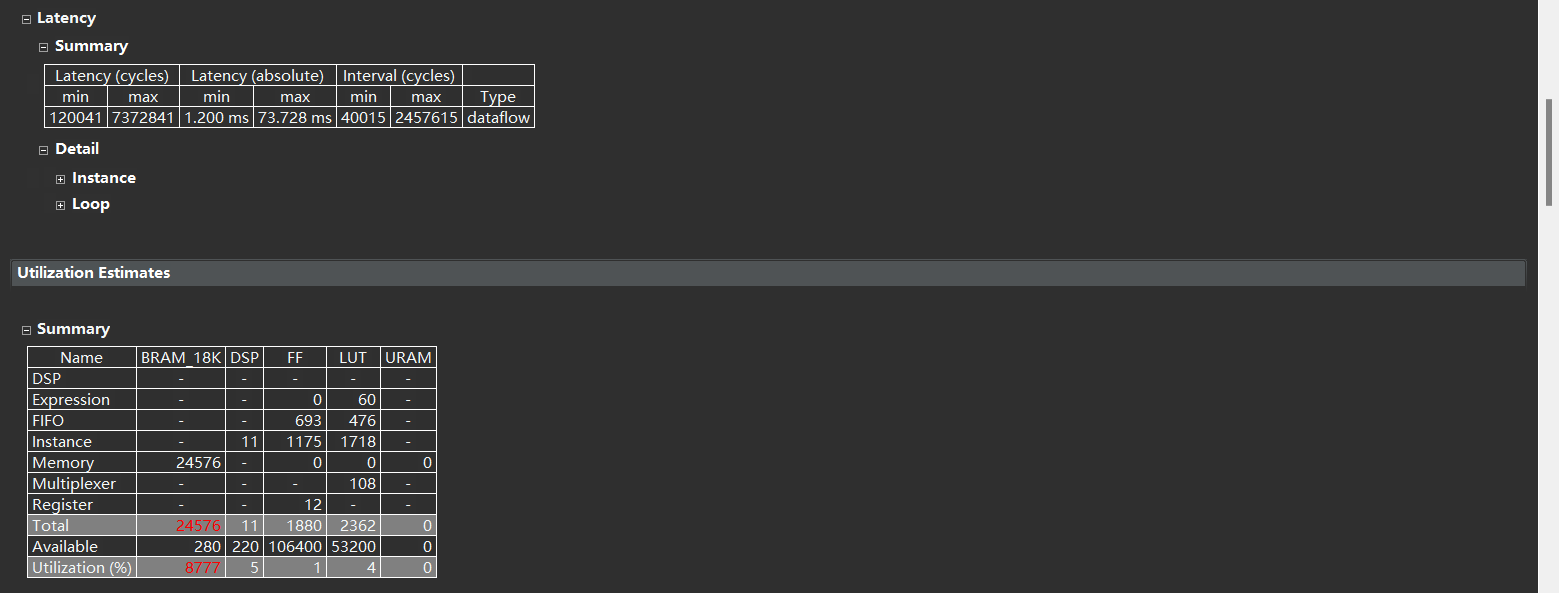
\includegraphics[width=\textwidth]{images/7.png}
        \caption{Performance and Resource estimate after \texttt{DATAFLOW} directive applied.}
    \end{figure}
    The Dataflow pipeline throughput indicates the number of clocks cycles between each set of input reads. If this throughput value is less than the design latency, it indicates the design can start processing new inputs before the current input data are output. While the overall latencies haven’t changed significantly, the dataflow throughput shows that the design can achieve close to the theoretical limit ($1920\times1280=2457600$) of processing one pixel every clock cycle. Take a screenshot of the Performance Estimates and Utilization Estimates of the Synthesis Details Report after \texttt{DATAFLOW} directive is applied.
    \item Scrolling down into the \textit{Utilization Estimates} section, observe that the number of BRAMs required has doubled. This is due to the default ping-pong buffering in the data flow. When DATAFLOW optimization is performed, memory buffers are automatically inserted between the functions to ensure the next function can begin operation before the previous function has finished. The default memory buffers are ping-pong buffers sized to accommodate the largest producer or consumer array fully. Vitis HLS allows the memory buffers to be the default ping-pong buffers or FIFOs. Since this design has data accesses that are fully sequential, FIFOs can be used. Another advantage to using FIFOs is that the size of the FIFOs can be directly controlled (not possible in ping-pong buffers where random accesses are allowed).
    \item The memory buffer type can be selected using the Vitis HLS Configuration command.
\end{enumerate}
Apply the Dataflow configuration command, generate the solution, and observe the improved resource utilization.
\begin{enumerate}
    \item Select Solution > Solution Settings... to access the configuration command settings.
    \item In the Solution Settings (solution3) dialog, General->Configuration Settings->Commands. Expand config\_dataflow, change default\_channel to "fifo" with fifo\_depth = 2, scalar\_fifo\_depth = 0, start\_fifo\_depth = 0, strict\_mode is warning.
    \item Run C Synthesis. If your resource estimate is still the same, see Appendix \ref{AFifo}. Note that the performance parameter has not changed; however, resource estimates show that the design is not using any BRAM, and other resources (FF, LUT) usage has also been reduced:
    \begin{figure}[H]
        \centering
        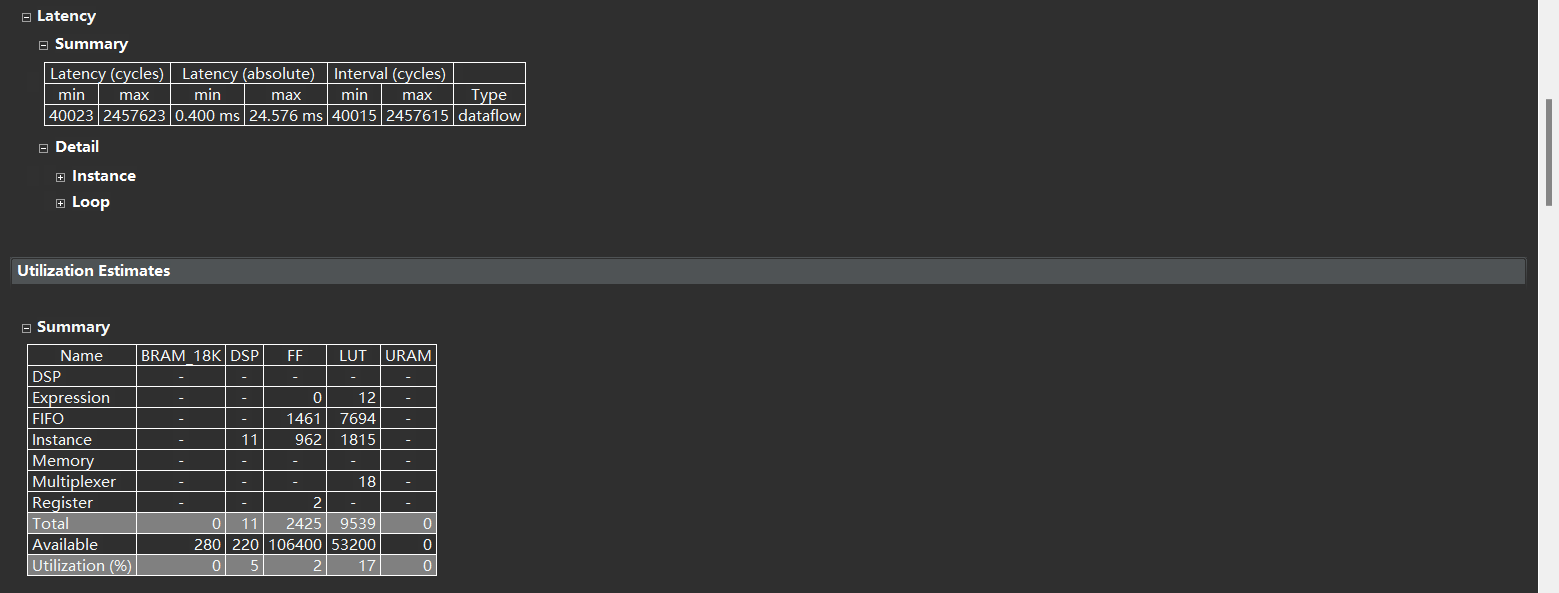
\includegraphics[width=\textwidth]{images/9.png}
        \caption{Resource estimation after Dataflow configuration command.}
    \end{figure}
    Take a screenshot of the Performance Estimates and Utilization Estimates of the Synthesis Details Report after configuring Dataflow commands.
\end{enumerate}
\subsection{(Optional) Export and implement the design in Vitis HLS}\label{S26}
In Vitis HLS, export the design, select Verilog as a language, and run the implementation by selecting Evaluate option.
\begin{enumerate}
    \item In Vitis HLS, select Solution > Export RTL to open the Export RTL dialog so the desired implementation can be run.
    \item Go to Solution Settings (solution3)->General->Configuration Settings->Commands->config\_export->rtl, choose either verilog or vhdl. Then, you have to go to Flow Navigator->IMPLEMENTATION->Run Implementation \cite{exportrtl}, in the pop-up window Run Implementation, select RTL Synthesis, Place \& Route, select RTL as Verilog or VHDL, and choose an IP location. These arguments are the same in solution settings. If you do not run the implementation first, Export RTL will automatically do the implementation, but it specifies RTL Synthesis only by default. If you get an error:
    \begin{minted}[breaklines,breakanywhere]{text}
ERROR: [IMPL 213-28] Failed to generate IP.  yuv_filter.prj:solution3
    \end{minted}
    see Appendix \ref{AImpl}. If your anti-virus software warns you that\\
    C:/Windows/SysWOW64/cscript.exe is executing target\\
    yuv\_filter.prj/solution3/impl/verilog/project.runs/bd\_0\_hls\_inst\_0\_synth\_1/rundef.js, ignore it. After the implementation finishes \cite{tclstack}, export the RTL. Take a screenshot of your implementation report.
\end{enumerate}
\subsection{Conclusion}
In this part, you learned that even though this design could not be pipelined at the top level, a strategy of pipelining the individual loops and then using dataflow optimization to make the functions operate in parallel was able to achieve the same high throughput, processing one pixel per clock. When the \texttt{DATAFLOW} directive is applied, the default memory buffers (of ping-pong type) are automatically inserted between the functions. Using the fact that the design used only sequential (streaming) data accesses allowed the costly memory buffers associated with dataflow optimization to be replaced with simple 2-element FIFOs using the Dataflow command configuration.

\newpage
\section{Implement and Optimize Discrete Cosine Transform}\label{S3}
\subsection{Discrete cosine transform}\label{dctintro}
A discrete cosine transform (DCT) expresses a finite sequence of data points in terms of a sum of cosine functions oscillating at different frequencies\cite{enwiki:1113261571}. In signal processing and data compression, the most important variants are what’s called DCT-II through DCT-IV. What’s commonly called “the” DCT is the DCT-II; this is the transform used in, among other things, JPEG, MPEG-1 and MPEG-2. The DCT-III is the inverse of the DCT-II (up to scaling, depending on how the two are normalized; there are different conventions in use). Thus it’s often called “the” IDCT (inverse DCT). The DCT-IV is its own inverse and forms the basis for the MDCT (modified DCT), a lapped transform that’s at the heart of most popular perceptual audio codecs (MP3, AAC, Vorbis, and Opus, among others) \cite{ryg}. DCT helps separate the image into parts (or spectral sub-bands) of differing importance (with respect to the image’s visual quality). DCT is similar to the discrete Fourier transform: it transforms a signal or image from the spatial domain to the frequency domain. To an image f, f(x,y) represents the pixel value at (x,y), the equation of the DCT transformation is \cite{488}:
\begin{equation}
    F(u,v)=\alpha(u)\alpha(v)\sum_{x=0}^{M-1}{\sum_{y=0}^{N-1}{f(x,y)\cos{\frac{(2x+1)u\pi}{2M}}\cos{\frac{(2y+1)v\pi}{2N}}}},
\end{equation}
where $u=0,1\dots.M-1,v=0,1\dots N-1$. $\alpha(u)=\left\{\begin{array}{ll}\frac{1}{\sqrt{M}}&u=0\\\sqrt{\frac{2}{M}}&u\neq0\end{array}\right.$ $\alpha(v)=\left\{\begin{array}{ll}\frac{1}{\sqrt{N}}&v=0\\\sqrt{\frac{2}{N}}&v\neq0\end{array}\right.$.

For most images, much of the signal energy lies at low frequencies; these appear in the upper left corner of the DCT. To reverse the image, the equation of the inverse DCT (iDCT) transformation is:
\begin{equation}
    f(x,y)=\sum_{u=0}^{M-1}{\sum_{v=0}^{N-1}{\alpha(u)\alpha(v)F(u,v)\cos{\frac{(2x+1)u\pi}{2M}}\cos{\frac{(2y+1)v\pi}{2N}}}},
\end{equation}
where $x=0,1\dots.M-1,y=0,1\dots N-1$. $\alpha(u)=\left\{\begin{array}{ll}\frac{1}{\sqrt{M}}&u=0\\\sqrt{\frac{2}{M}}&u\neq0\end{array}\right.$ $\alpha(v)=\left\{\begin{array}{ll}\frac{1}{\sqrt{N}}&v=0\\\sqrt{\frac{2}{N}}&v\neq0\end{array}\right.$.
If the input image is square, another way is to use DCT (basis) (transform) matrix, which is much faster. The M-by-M transform matrix T is given by
\begin{equation}
    T_{pq}=\left\{\begin{array}{lll}\frac{1}{\sqrt{M}}&p=0,&0\leq q\leq M-1\\\sqrt{\frac{2}{M}}\cos{\frac{\pi(2q+1)p}{2M}}&1\leq p\leq M-1,&0\leq q\leq M-1\end{array}\right.
\end{equation}
For an M-by-M matrix A, T*A is an M-by-M matrix whose columns contain the one-dimensional DCT of the columns of A. The two-dimensional DCT of A can be computed as B=T*A*T'. Since T is a real orthonormal matrix, its inverse is the same as its transpose. Therefore, the inverse two-dimensional DCT of B is given by T'*B*T \cite{dctdoc}.

The sample MATLAB code is:
\inputminted{matlab}{compression_test.m}

The Fourier DCT matrix can also be applied. The rows of the Fourier DCT matrix are basis sequences of the DCT. The DCT matrix of type 2 has an inverse of type 3. Each entry $F_{rs}$ of an $n\times n$ DCT matrix of type 2 is computed as \cite{fdctmdoc}:
\begin{equation}
    \frac{1}{\sqrt{n}}\cos{\left(\frac{\pi}{n}\left(r-\frac{1}{2}\right)\left(s-1\right)\right)}
\end{equation}
Each entry $F_{rs}$ of the DCT matrix of type 3 is computed as:
\begin{equation}
    \frac{1}{\sqrt{n}}\left\{\begin{array}{ll}1&r=1\\2\cos{\left(\frac{\pi}{n}\left(r-1\right)\left(s-\frac{1}{2}\right)\right)}&r=2,\dots,n\end{array}\right.
\end{equation}

The sample Wolfram Mathematica code is:
\lstinputlisting[language=Mathematica]{compression_test_clean.nb}

The sample Python code is:
\begin{minted}[breaklines,breakanywhere,linenos]{python}
import numpy as np

def DCT_basis(M):
    dct_basis = np.zeros((M, M))
    dct_basis[0,:] = 1 / np.sqrt(M)
    for p in range(1,M):
        for q in range(M):
            dct_basis[p, q] = np.sqrt(2 / M) * np.cos(np.pi * (2 * q + 1) * p / (2 * M))
    
    return dct_basis


def DCT_transform(img):
    H,W = img.shape
    if H != W:
        img_dct = np.zeros((H, W))
        for u in range(H):
            for v in range(W):
                img_dct[u, v] = 0
                for x in range(H):
                    for y in range in range(W):
                        if u == 0 and v == 0:
                            img_dct[u, v] += 1 / np.sqrt(H * W) * img[x, y]
                        elif u == 0:
                            img_dct[u, v] += np.sqrt(2 / H * W) * img[x, y] * np.cos(((2 * y + 1) * v * np.pi) / (2 * W))
                        elif v == 0:
                            img_dct[u, v] += np.sqrt(2 / H * W) * img[x, y] * np.cos(((2 * x + 1) * u * np.pi) / (2 * H))
                        else:
                            img_dct[u, v] += 2 / np.sqrt(H * W) * img[x, y] * np.cos(((2 * x + 1) * u * np.pi) / (2 * H)) * np.cos(((2 * y + 1) * v * np.pi) / (2 * W))
    else:
        dct_basis = DCT_basis(W)
        img_dct = dct_basis @ img @ np.transpose(dct_basis)
    
    return img_dct


def iDCT_transform(img_dct):
    H,W = img_dct.shape
    if H != W:
        img_recover = np.zeros((H, W))
        for x in range(H):
            for y in range(W):
                img_recover[x, y] = 0
                for u in range(H):
                    for v in range in range(W):
                        if u == 0 and v == 0:
                            img_recover[x, y] += 1 / np.sqrt(H * W) * img_dct[u, v]
                        elif u == 0:
                            img_recover[x, y] += np.sqrt(2 / H * W) * img_dct[u, v] * np.cos(((2 * y + 1) * v * np.pi) / (2 * W))
                        elif v == 0:
                            img_recover[x, y] += np.sqrt(2 / H * W) * img_dct[u, v] * np.cos(((2 * x + 1) * u * np.pi) / (2 * H))
                        else:
                            img_recover[x, y] += 2 / np.sqrt(H * W) * img_dct[u, v] * np.cos(((2 * x + 1) * u * np.pi) / (2 * H)) * np.cos(((2 * y + 1) * v * np.pi) / (2 * W))
    else:
        dct_basis = DCT_basis(W)
        img_recover = np.transpose(dct_basis) @ img_dct @ dct_basis
    
    return img_recover
\end{minted}
One of the properties of the 2-D DCT is that it is separable, meaning that it can be separated into a pair of 1-D DCTs. To obtain the 2-D DCT of a block, a 1-D DCT is first performed on the rows of the block then a 1-D DCT is performed on the columns of the resulting block \cite{l11}.
% \begin{equation}
%     Z(w,v)=\alpha(v)\sum_{y=0}^{N-1}{f(x,y)\cos{\frac{(2y+1)w\pi}{2}}
% \end{equation}
\begin{figure}[H]
    \centering
    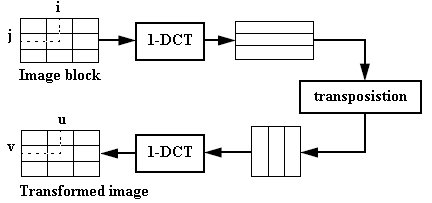
\includegraphics[width=\textwidth]{images/11.jpg}
    \caption{Computation of 2-D DCT using separability property \cite{5227881}.}
\end{figure}
The same applies to the IDCT. A 2-D DCT can be separated by applying 1-D DCT (vertically) to columns and then applying 1-D DCT (horizontally) to resultant vertical DCT, or equivalently, applying 1-D DCT (horizontally) to rows and then applying 1-D DCT (vertically) to resultant horizontal DCT. A simple MATLAB script can be used for verification:
\inputminted[linenos]{matlab}{dct_opt.m}
\subsection{Validate your design from Vitis HLS command line}\label{S32}
\begin{enumerate}
    \item Prepare your \texttt{input.dat} from the top-left corner $8\times8$ block of \texttt{lab3\_starter/lena\_\\
    gray.bmp}. You can also use \texttt{lab3\_starter/lena\_gray.raw}, which is the binary of all the points of the bitmap (BMP) file.
    \item Denote the DCT basis matrix as $T$. Prepare your \texttt{dct\_coeff\_table.txt} as a matrix $C$ by
    \begin{equation}
        C_{i,j}=\mathrm{round}(2^{\mathrm{CONST\_BITS}+1.5}T_{i,j})
    \end{equation}
    \item Run \texttt{make} by \texttt{lab3\_starter/dct/Makefile}.
\end{enumerate}
\subsection{Create a new project}\label{S33}
\begin{enumerate}
    \item Create a new Vitis HLS project named \textbf{dct} with the top function \texttt{dct} and the xc7z020clg400-1 part.
    \item Add \texttt{lab3\_starter/dct.c} as the Source and add Add \texttt{lab3\_starter/dct\_test.c} as the Test Bench.
    \item The top-level function \texttt{dct}, is defined at line 78. It implements a 2D DCT algorithm by first processing each row of the input array via a 1D DCT then processing the columns of the resulting array through the same 1D DCT. It calls \texttt{read\_data}, \texttt{dct\_2d}, and \texttt{write\_data} functions.\\
    The \texttt{read\_data} function is defined at line 54 and consists of two loops – RD\_Loop\_Row and RD\_Loop\_Col. The \texttt{write\_data} function is defined at line 66 and consists of two loops to perform writing the result. The \texttt{dct\_2d} function, defined at line 23, calls \texttt{dct\_1d} function and performs transpose.\\
    Finally, \texttt{dct\_1d} function, defined at line 4, uses \texttt{dct\_coeff\_table} and performs the required function by implementing a basic iterative form of the 1D Type-II DCT algorithm. The following figure shows the function hierarchy on the left-hand side, the loops in the order they are executed, and the flow of data on the right-hand side.
    \begin{figure}[H]
        \centering
        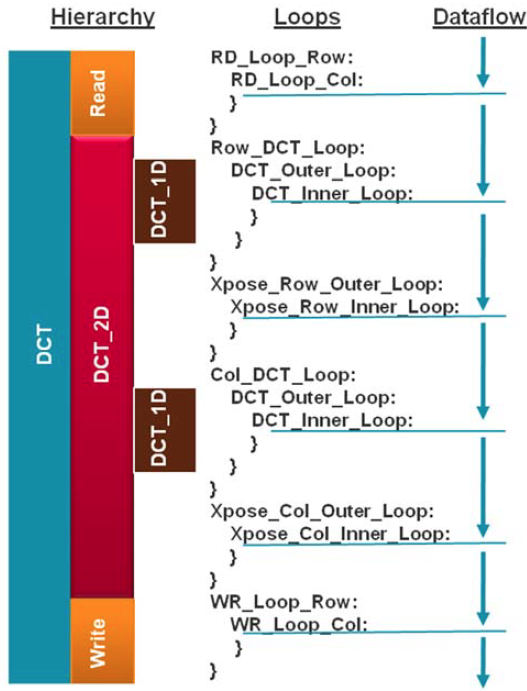
\includegraphics[width=\textwidth]{images/12.png}
        \caption{Design hierarchy and dataflow.}
    \end{figure}
\end{enumerate}
\subsection{Apply \texttt{PIPELINE} Directive}\label{S34}
Synthesize the design with the defaults. View the synthesis results and answer the question listed in the detailed section of this step. Run the Co-simulation, selecting Verilog. Verify that the simulation passes. Apply the PIPELINE directive to DCT\_Inner\_Loop, Xpose\_Row\_Inner\_Loop, Xpose\_Col\_Inner\_Loop, RD\_Loop\_Col, and WR\_Loop\_Col. Generate the solution and analyze the output. Create a new solution by copying the previous solution settings. 

\begin{enumerate}
    \item Explicitly add the HLS PIPELINE directive for dct\_1d->DCT\_Outer\_Loop->\\
    DCT\_Inner\_Loop, because Vitis HLS will automatically pipeline loop RD\_Loop\_Col, WR\_Loop\_Col, Xpose\_Row\_Inner\_Loop, Xpose\_Col\_Inner\_Loop, and\\
    DCT\_Outer\_Loop, but we want to pipeline DCT\_Inner\_Loop rather than DCT\_\\
    Outer\_Loop.
    \item Run C Synthesis.
    \item When synthesis is completed, several report files will become accessible, and the Synthesis Results will be displayed in the information pane.% Note that the Synthesis Report section in the Explorer view only shows dct\_1d.rpt, dct\_2d.rpt, and dct.rpt entries. The \texttt{read\_data} and \texttt{write\_data} functions reports are not listed. This is because these two functions are inlined. Verify this by scrolling up into the Vitis HLS Console view.
    \item The Synthesis Report shows the performance and resource estimates as well as estimated latency in the design. Report the following metrics of the \texttt{dct} function:
    \begin{enumerate}
        \item Estimated clock period
        \item Worst case latency
        \item Number of DSP48E used
        \item Number of BRAMs used
        \item Number of FFs used
        \item Number of LUTs used
    \end{enumerate}
    \item The report also shows the top-level interface signals generated by the tools.
    \begin{figure}[H]
        \centering
        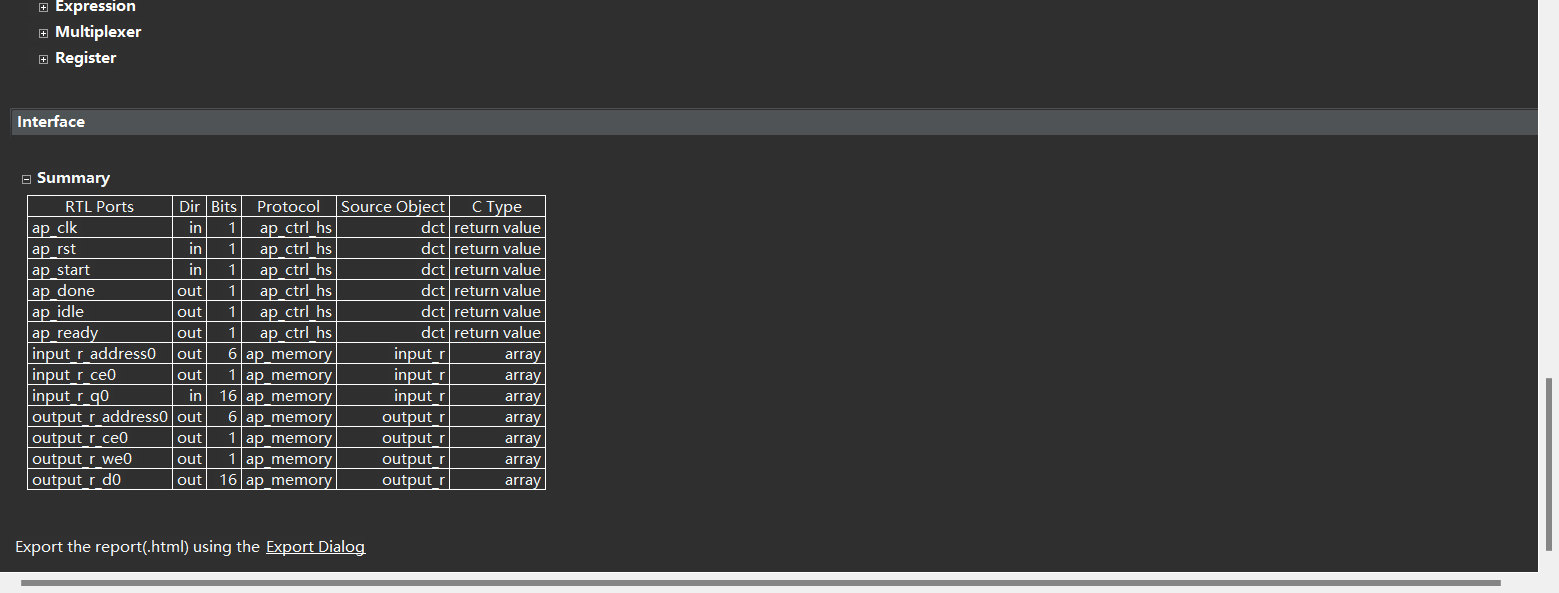
\includegraphics[width=\textwidth]{images/13.png}
        \caption{Generated interface signals.}
    \end{figure}
    You can see ap\_clk, ap\_rst are automatically added. The ap\_start, ap\_done, ap\_idle, and ap\_ready are top-level signals used as handshaking signals to indicate when the design is able to accept next computation command (ap\_idle), when the next computation is started (ap\_start), and when the computation is completed (ap\_done). The top-level function has input and output arrays; hence an ap\_memory interface is generated for each of them.
    \item Run C Cosimulation. You can now inspect your generated \texttt{output.dat}.
    \item In the Module Hierarchy pane, select the dct entry and observe the\\
    RD\_Loop\_Row\_RD\_Loop\_Col and WR\_Loop\_Row\_WR\_Loop\_Col entries in the Schedule Viewer. These are two nested loops flattened and given the new names formed by appending the inner loop name to the outer loop name. You can also verify this by looking in the Console view message. If it is
    \begin{minted}[breaklines,breakanywhere,linenos]{text}
INFO: [XFORM 203-541] Flattening a loop nest 'RD_Loop_Row' (../lab3_starter/dct/dct.c:56:8) in function 'dct'.
WARNING: [HLS 200-960] Cannot flatten loop 'DCT_Outer_Loop' (../lab3_starter/dct/dct.c:6:17) in function 'dct' the outer loop is not a perfect loop because there is nontrivial logic in the loop latch.
Resolution: For help on HLS 200-960 see www.xilinx.com/cgi-bin/docs/rdoc?v=2022.1;t=hls+guidance;d=200-960.html
INFO: [XFORM 203-541] Flattening a loop nest 'Row_DCT_Loop' (../lab3_starter/dct/dct.c:28:13) in function 'dct'.
INFO: [XFORM 203-541] Flattening a loop nest 'Xpose_Row_Outer_Loop' (../lab3_starter/dct/dct.c:28:16) in function 'dct'.
WARNING: [HLS 200-960] Cannot flatten loop 'DCT_Outer_Loop' (../lab3_starter/dct/dct.c:6:17) in function 'dct' the outer loop is not a perfect loop because there is nontrivial logic in the loop latch.
Resolution: For help on HLS 200-960 see www.xilinx.com/cgi-bin/docs/rdoc?v=2022.1;t=hls+guidance;d=200-960.html
INFO: [XFORM 203-541] Flattening a loop nest 'Col_DCT_Loop' (../lab3_starter/dct/dct.c:28:13) in function 'dct'.
INFO: [XFORM 203-541] Flattening a loop nest 'Xpose_Col_Outer_Loop' (../lab3_starter/dct/dct.c:28:16) in function 'dct'.
INFO: [XFORM 203-541] Flattening a loop nest 'WR_Loop_Row' (../lab3_starter/dct/dct.c:68:8) in function 'dct'.
    \end{minted}
    then you are correct. If it is
    \begin{minted}[breaklines,breakanywhere,linenos]{text}
INFO: [XFORM 203-541] Flattening a loop nest 'RD_Loop_Row' (../lab3_starter/dct/dct.c:56:8) in function 'dct'.
INFO: [XFORM 203-541] Flattening a loop nest 'Row_DCT_Loop' (../lab3_starter/dct/dct.c:28:13) in function 'dct'.
INFO: [XFORM 203-541] Flattening a loop nest 'Xpose_Row_Outer_Loop' (../lab3_starter/dct/dct.c:28:16) in function 'dct'.
INFO: [XFORM 203-541] Flattening a loop nest 'Col_DCT_Loop' (../lab3_starter/dct/dct.c:28:13) in function 'dct'.
INFO: [XFORM 203-541] Flattening a loop nest 'Xpose_Col_Outer_Loop' (../lab3_starter/dct/dct.c:28:16) in function 'dct'.
INFO: [XFORM 203-541] Flattening a loop nest 'WR_Loop_Row' (../lab3_starter/dct/dct.c:68:8) in function 'dct'.
    \end{minted}
    then you are incorrect.
    \item Click the "Open Viewer" button in the top bar. It will open the Schedule Viewer by default.
    \begin{figure}[H]
        \centering
        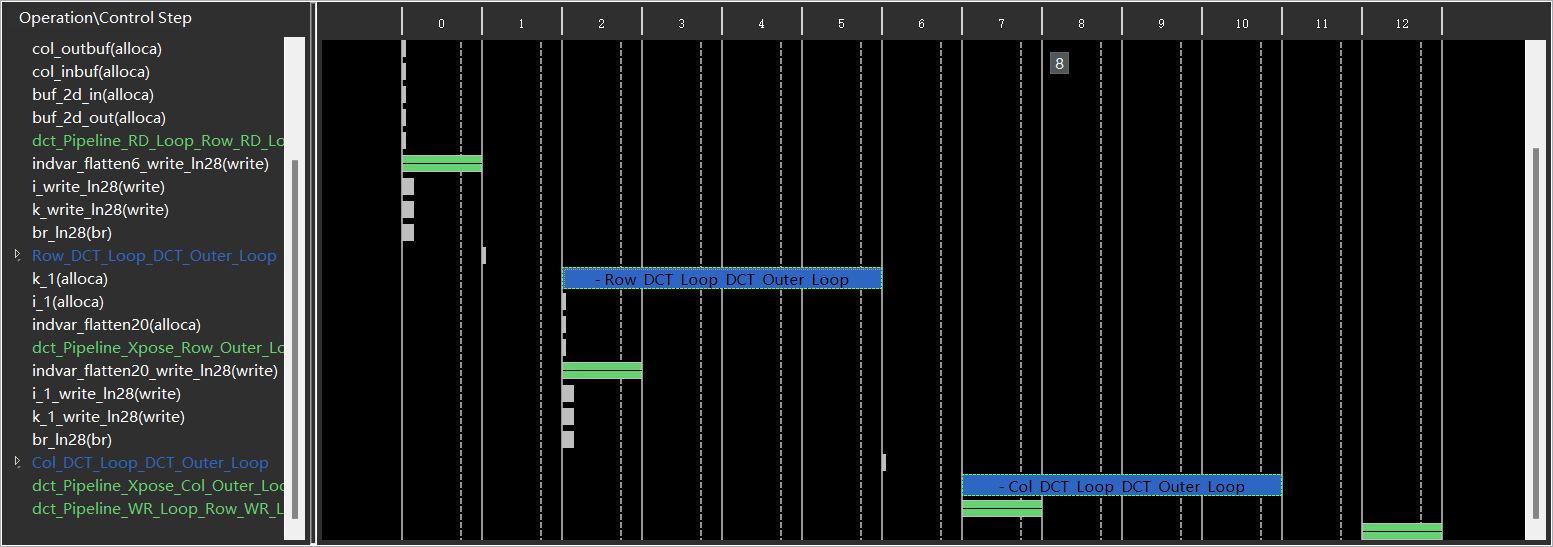
\includegraphics[width=\textwidth]{images/14.png}
    \end{figure}
    You can see that most cycle time is cost by Row\_DCT\_Loop\_DCT\_Outer\_Loop and Col\_DCT\_Loop\_DCT\_Outer\_Loop, which are mainly cost by\\
    dct\_Pipeline\_DCT\_Inner\_Loop and dct\_Pipeline\_DCT\_Inner\_Loop1 respectively. You can furthermore expand the DCT\_Inner\_Loop of them and observe that most cycle time is cost by coeff(read), buf\_2d\_in\_load(read), mul\_ln17(*), and tmp\_4(+). You can right-click on the Operation/Control Step and click "Goto Source", then a "C Source" tab will show in the bottom perspective. Use up and down key to browse the operations/control steps with their source.
    \begin{figure}[H]
        \centering
        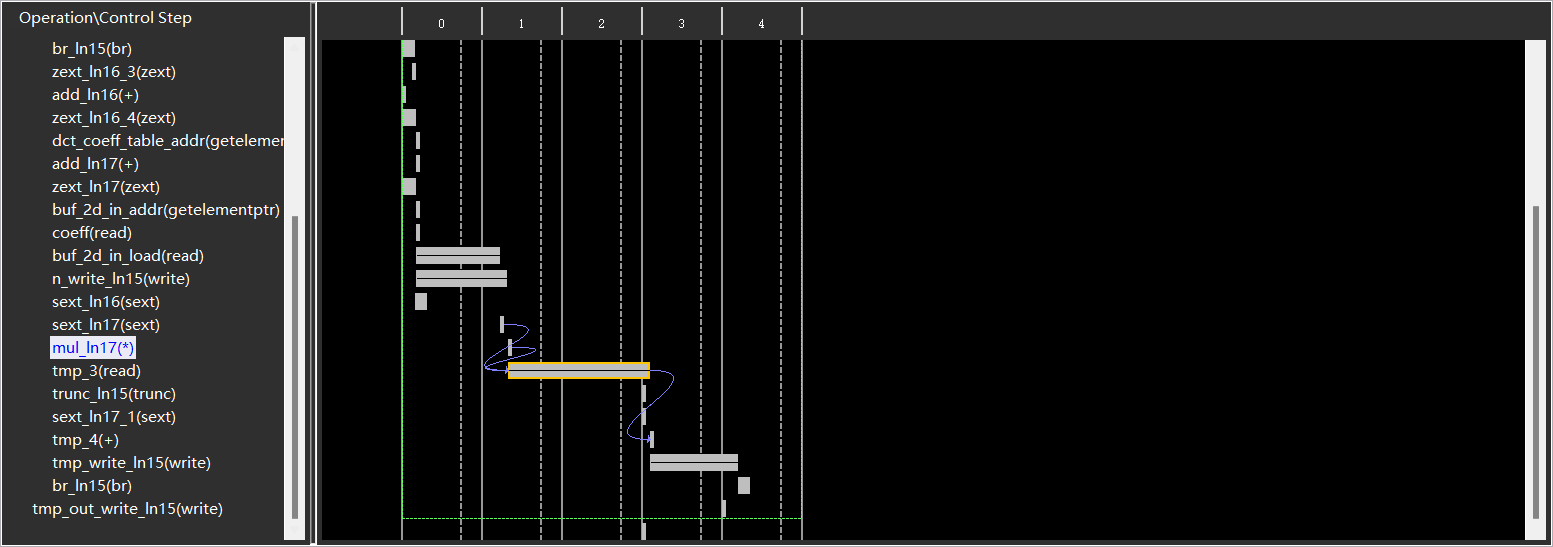
\includegraphics[width=\textwidth]{images/15.png}
    \end{figure}
    Line 19 is not operated by dct\_Pipeline\_DCT\_Inner\_Loop or\\
    dct\_Pipeline\_DCT\_Inner\_Loop1. Line 19 is scheduled after they finish.
    \begin{figure}[H]
        \centering
        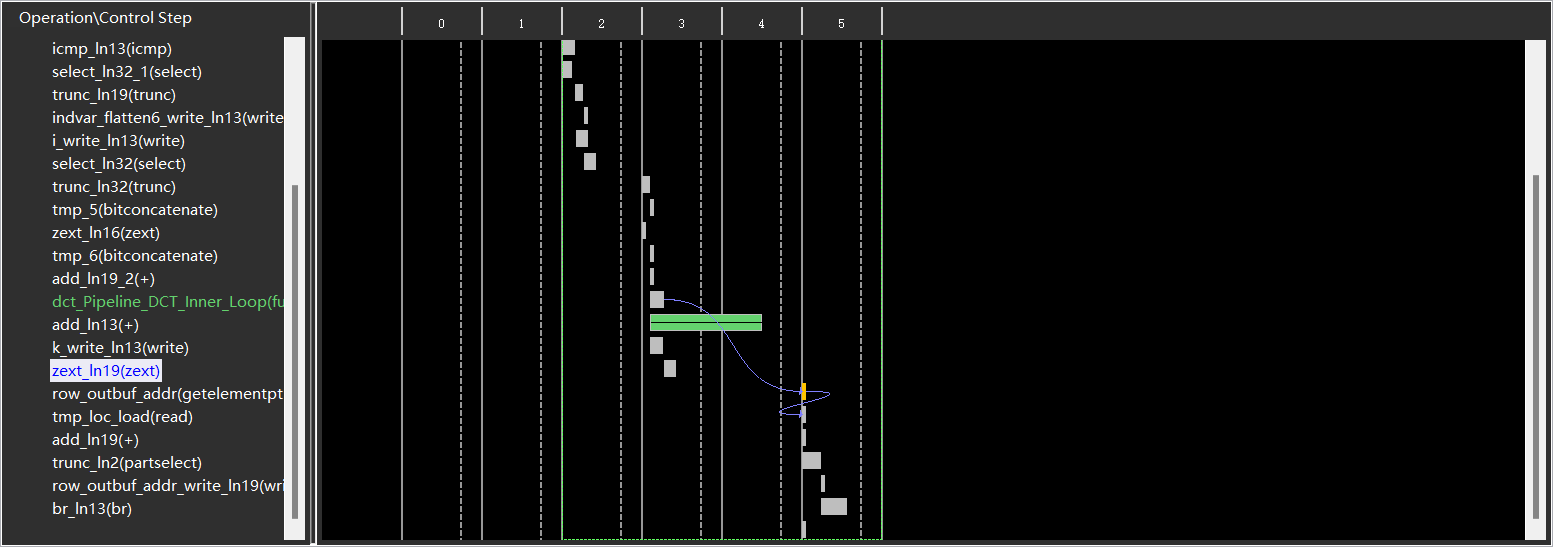
\includegraphics[width=\textwidth]{images/16.png}
    \end{figure}
    \item Create a new solution solution2 from solution1. Remove the HLS PIPELINE directive of DCT\_Inner\_Loop to allow auto-pipelining of DCT\_Outer\_Loop.
    \item Run C Synthesis for solution2.
    \item Generate the Vitis HLS Report Comparison between solution1 and solution2. Take a screenshot of the Performance Estimates and the Utilization Estimates.
    \item Note that different from solution1, in the Utilization Estimates section of the Synthesis Details(solution2)(dct\_csynth.rpt), expand Detail->Memory, the coefficient table was automatically partitioned, resulting in 8 separate ROMs: this helped reduce the latency by keeping the unrolled computation loop fed; however, the input arrays to the \texttt{dct\_1d} function were not automatically partitioned, and the \texttt{dct\_1d} function utilize more resources. In the Console view, you can also see one line:
    \begin{minted}[breaklines,breakanywhere,linenos]{text}
INFO: [XFORM 203-102] Partitioning array 'dct_coeff_table' in dimension 2 automatically.
    \end{minted}
    \begin{figure}[H]
        \centering
        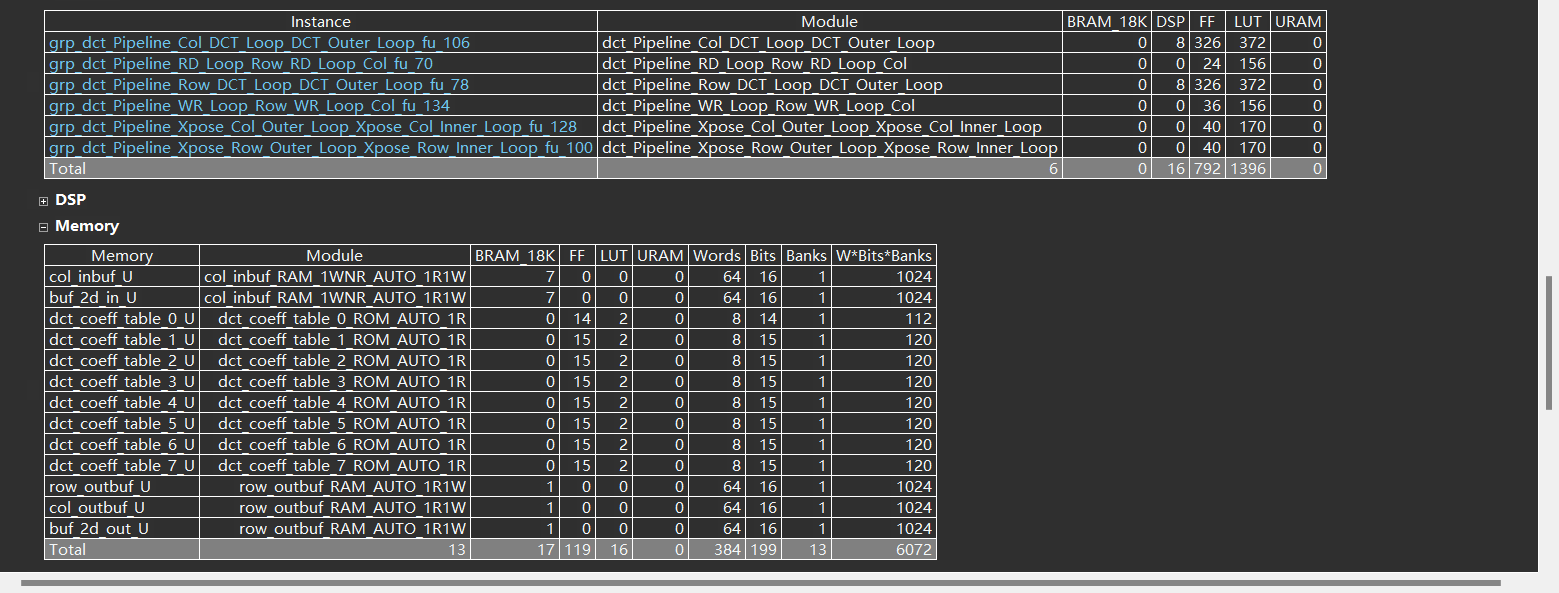
\includegraphics[width=\textwidth]{images/17.png}
        \caption{Automatic partitioning of \texttt{dct\_coeff\_table}.}
    \end{figure}
    In the Schedule Viewer, we can see the partitioned \texttt{dct\_coeff\_table} pipelining read and getelement.
    \begin{figure}[H]
        \centering
        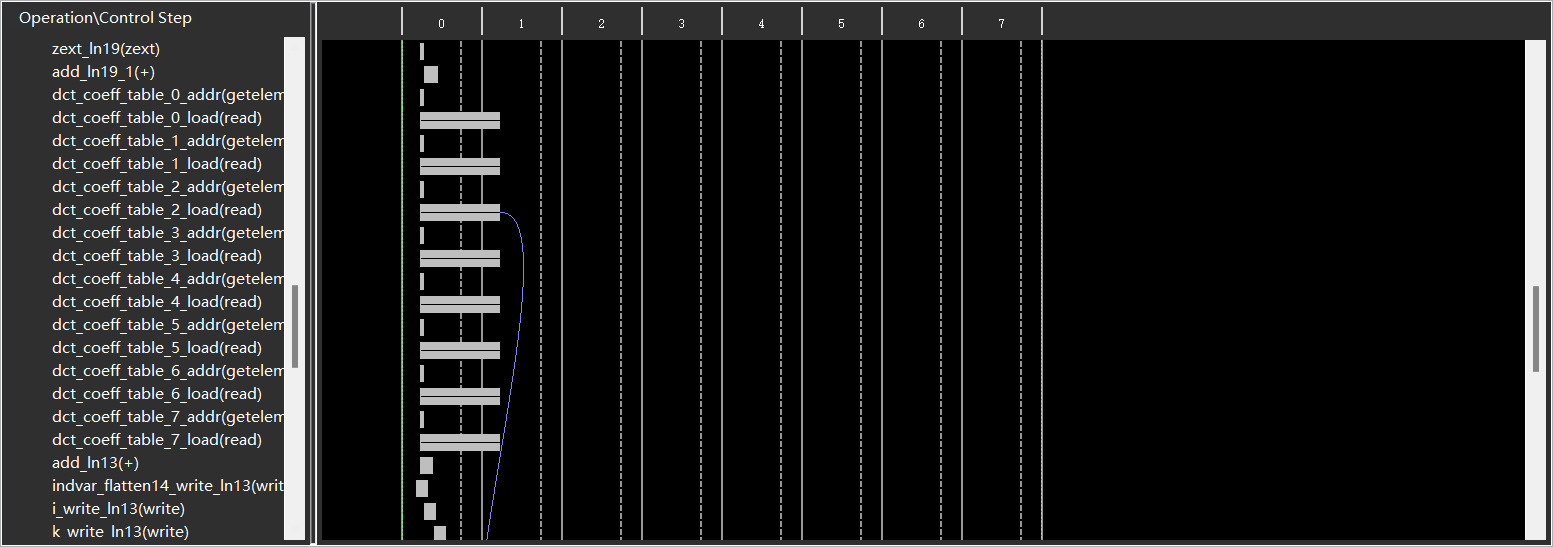
\includegraphics[width=\textwidth]{images/18.png}
        \caption{The Performance view of the (Row\_DCT\_Loop\_)DCT\_Outer\_Loop function.}
    \end{figure}
\end{enumerate}
\subsection{Improve memory bandwidth}\label{S35}
Create a new solution by copying the previous solution (solution2) settings. Apply the \texttt{ARRAY\_PARTITION} directive to \texttt{buf\_2d\_in} of \texttt{dct} (since the bottleneck was on src port of the \texttt{dct\_1d} function, which was passed via \texttt{in\_block} of the \texttt{dct\_2d} function, which in turn was passed via \texttt{buf\_2d\_in} of the \texttt{dct} function) and \texttt{col\_inbuf} of \texttt{dct\_2d}. Generate the solution.
\begin{enumerate}
    \item Create a new solution solution3 from solution2.
    \item Add the \texttt{ARRAY\_PARTITION} directive to \texttt{buf\_2d\_in} of \texttt{dct}. Specify dim = 2, type is complete. Similarly, apply the \texttt{ARRAY\_PARTITION} directive with dimension of 2 to the \texttt{col\_inbuf} array.
    \item Run C Synthesis.
    \item When the synthesis is completed, select Project > Compare Reports... to compare the two solutions. Observe that the latency is reduced. Scroll down in the comparison report to view the resource utilization. Observe the increase in FF resource utilization.
    \begin{figure}[H]
        \centering
        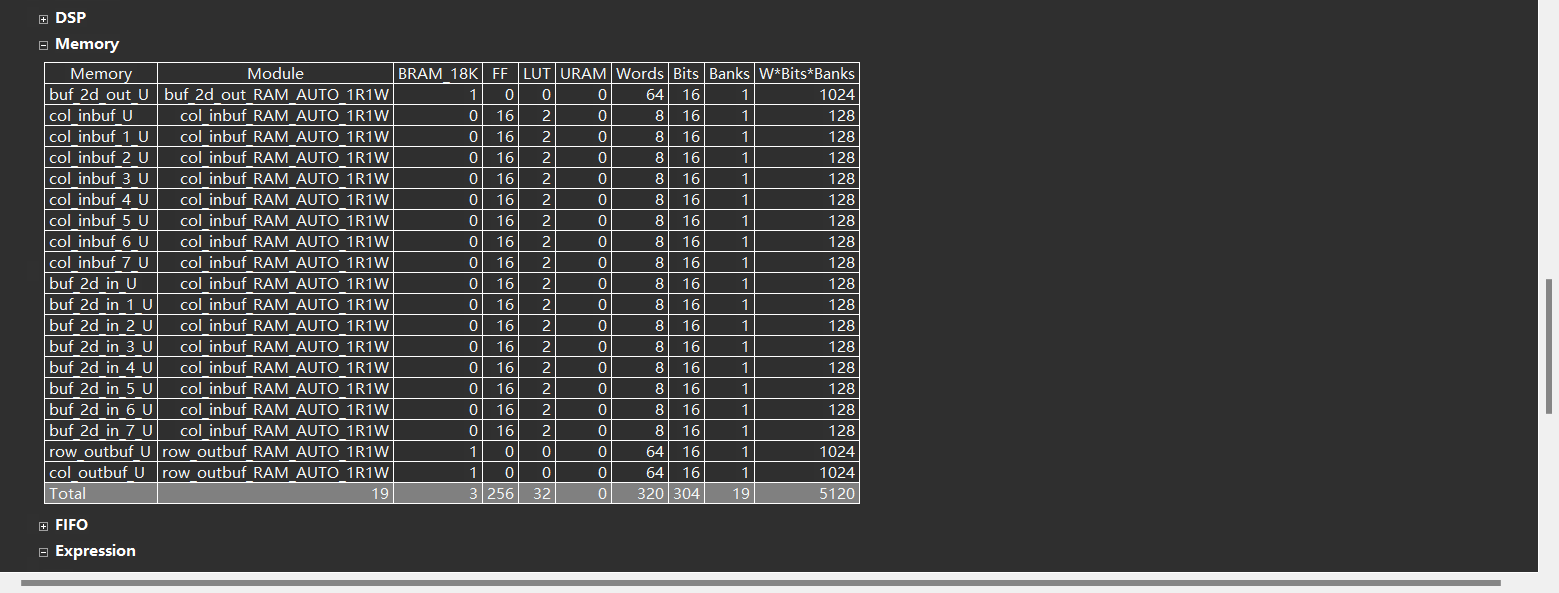
\includegraphics[width=\textwidth]{images/19.png}
        \caption{Resource profile after partitioning buffers.}
    \end{figure}
    \item In the Utilization Estimates section of the Synthesis Details(solution3)(dct\_csynth.rpt), expand Detail->Memory, and observe that most of the resources are consumed by instances. The \texttt{buf\_2d\_in} array is partitioned into multiple memories, and most of the operations are done in addition and comparison. Take a screenshot of the utilization estimates detail of memory.
\end{enumerate}
\subsection{Apply \texttt{DATAFLOW} Directive}\label{S36}
Create a new solution solution4 by copying the previous solution (solution3) settings. Apply the \texttt{DATAFLOW} directive to the \texttt{dct} function to improve the throughput. Run C Synthesis. Generate the solution and analyze the output.

In the Synthesis Details, the Dataflow pipeline throughput indicates the number of clock cycles between each set of input reads (interval parameter). If this value is less than the design latency, it indicates the design can start processing new inputs before the current input data are output. Note that the dataflow is only supported for the functions and loops at the top level, not those
which are down through the design hierarchy. Only loops and functions exposed at the top level of the design will get benefit from dataflow optimization.

Compare solution3 and solution4. Observe that the latency is reduced. Scroll down into the Area Estimates, and observe that the number of BRAM\_18K required at the top level remained at 3. Observe that most of the latency and interval (throughput) is caused by the \texttt{dct\_2d} function. The interval of the top-level function \texttt{dct}, is less than the sum of the intervals of the \texttt{read\_data}, \texttt{dct\_2d}, and \texttt{write\_data} functions indicating that they operate in parallel and \texttt{dct\_2d} is the limiting factor.% From the Performance \& Resource Estimates section of the Synthesis summary(solution4), expand dct\_2d, it can be seen that \texttt{dct\_2d} is not operating in parallel as Row\_DCT\_Loop and Col\_DCT\_Loop were not pipelined.
\begin{minted}[breaklines,breakanywhere,linenos]{text}
INFO: [XFORM 203-712] Applying dataflow to function 'dct' (../lab3_starter/dct/dct.c:9:1), detected/extracted 3 process function(s): 
	 'read_data.1'
	 'dct_2d'
	 'write_data.1'.
INFO: [XFORM 203-11] Balancing expressions in function 'dct_2d' (../lab3_starter/dct/dct.c:17:7)...124 expression(s) balanced.
INFO: [HLS 200-111] Finished Loop, function and other optimizations: CPU user time: 0 seconds. CPU system time: 0 seconds. Elapsed time: 0.383 seconds; current allocated memory: 1.421 GB.
INFO: [XFORM 203-541] Flattening a loop nest 'WR_Loop_Row' (../lab3_starter/dct/dct.c:68:8) in function 'write_data.1'.
INFO: [XFORM 203-541] Flattening a loop nest 'RD_Loop_Row' (../lab3_starter/dct/dct.c:56:8) in function 'read_data.1'.
INFO: [XFORM 203-541] Flattening a loop nest 'Xpose_Row_Outer_Loop' (../lab3_starter/dct/dct.c:28:16) in function 'dct_2d'.
INFO: [XFORM 203-541] Flattening a loop nest 'Xpose_Col_Outer_Loop' (../lab3_starter/dct/dct.c:28:16) in function 'dct_2d'.
\end{minted}
\begin{figure}[H]
    \centering
    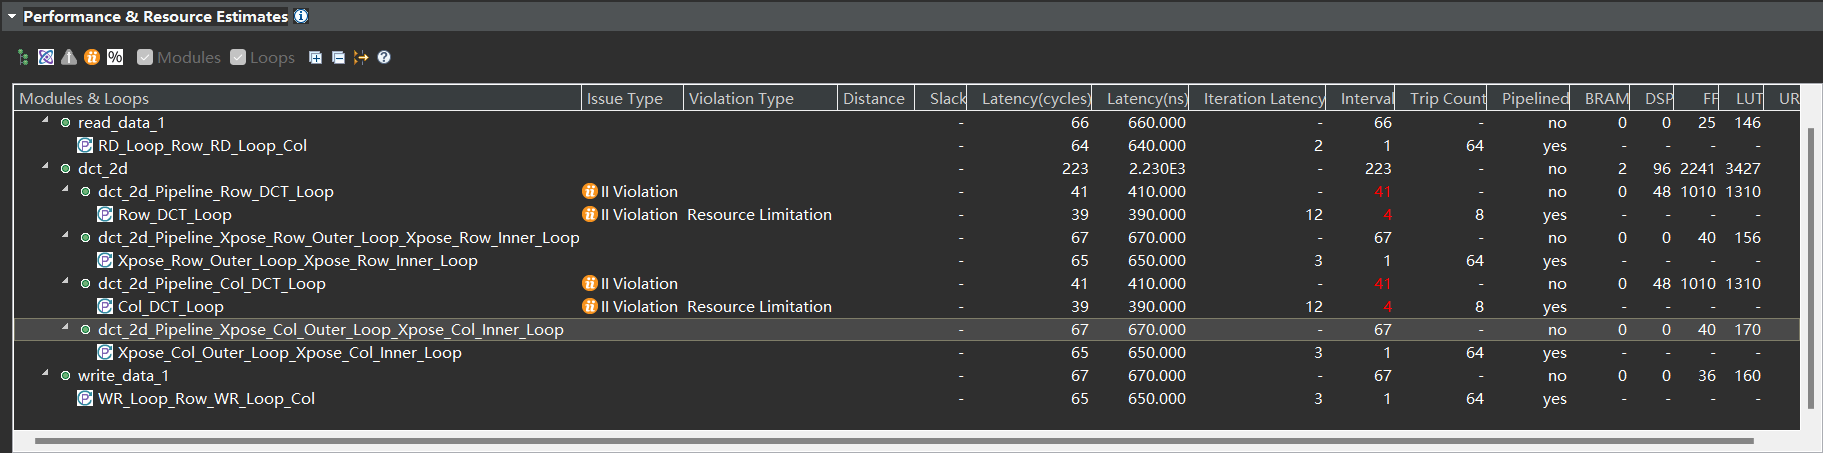
\includegraphics[width=\textwidth]{images/20.png}
    \caption{Performance analysis after the \texttt{DATAFLOW} directive.}
\end{figure}
One of the limitations of dataflow optimization is that it only works on top-level loops and functions. One way to have the blocks in \texttt{dct\_2d} operate in parallel would be to pipeline the entire function. This, however, would unroll all the loops and can sometimes lead to a large area increase. An alternative is to raise these loops up to the top level of the hierarchy, where dataflow optimization can be applied, by removing the \texttt{dct\_2d} hierarchy, i.e. inline the \texttt{dct\_2d} function.

\subsection{Apply \texttt{INLINE} Directive}\label{S37}
Create a new solution solution5 by copying the previous solution (solution4) settings. Apply \texttt{INLINE} directive to \texttt{dct\_2d}. Run C Synthesis. Generate the solution and analyze the output.

In the Console view, observe that
\begin{minted}[breaklines,breakanywhere,linenos]{text}
INFO: [XFORM 203-712] Applying dataflow to function 'dct' (../lab3_starter/dct/dct.c:9:1), detected/extracted 6 process function(s): 
	 'read_data.1'
	 'Loop_Row_DCT_Loop_proc'
	 'Loop_Xpose_Row_Outer_Loop_proc'
	 'Loop_Col_DCT_Loop_proc'
	 'Loop_Xpose_Col_Outer_Loop_proc'
	 'write_data.1'.
\end{minted}
Compare solution4 and solution5. Observe that the latency is reduced. Switch to the Analysis perspective, expand the Module Hierarchy entries, and select the \texttt{dct} entry. Observe that the \texttt{dct\_2d} entry is now replaced with Loop\_Row\_DCT\_Loop\_proc, Loop\_Xpose\_Row\_Outer\_Loop\_proc, Loop\_Col\_DCT\_Loop\_proc, and\\
Loop\_Xpose\_Col\_Outer\_Loop\_proc since the \texttt{dct\_2d} function is inlined. BRAM usage has increased once again (from 3 to 5), due to ping-pong buffering between more dataflow processes.

Compare all five solutions and take a screenshot of the Performance Estimates and the Utilization Estimates.
\subsection{Conclusion}\label{S3Con}
In this lab, you learned various techniques to improve performance and balance resource utilization. The PIPELINE directive that is applied to the outer loop will automatically cause the inner loop to unroll. When a loop is unrolled, resource utilization increases as operations are done concurrently. Partitioning memory may improve performance but will increase BRAM utilization. When the INLINE directive is applied to a function, the lower-level hierarchy is automatically dissolved. When the DATAFLOW directive is applied, the
default memory buffers (of ping-pong type) are automatically inserted between the top-level functions and loops. The Analysis perspective and console logs can provide insight into what is going on.
\subsection{Inverse discrete cosine transform (IDCT)}\label{S3idct}
\begin{enumerate}
    \item Write three new functions based on Section \ref{dctintro}:
    \begin{itemize}
        \item \texttt{void idct\_1d(dct\_data\_t src[DCT\_SIZE], dct\_data\_t dst[DCT\_SIZE])}
        \item \texttt{void idct\_2d(dct\_data\_t in\_block[DCT\_SIZE][DCT\_SIZE], dct\_data\_t\\
        out\_block[DCT\_SIZE][DCT\_SIZE])}
        \item \texttt{void idct(short input[N], short output[N])} 
    \end{itemize}
    \item In \texttt{dct\_test.c}, uncomment Line 20 \texttt{idct(b,c)} and print the array \texttt{short c[N]} to \texttt{output.dat}.
    \item Run \texttt{make}.
    \item (Optional) Re-generate \texttt{input.dat} of the full \texttt{lena\_gray.bmp} block-by-block. Process DCT and IDCT on each $8\times8$ block. Compose the transformed block into a recovered image.
\end{enumerate}

\newpage
\section{(Optional) JPEG and DCT Further On}\label{Sopt1}
\subsection{Introduction to JPEG}
JPEG (Joint Photographic Experts Group) is a commonly used method of lossy compression for digital images, particularly for those images produced by digital photography. JPEG compression is used in a number of image file formats. JPEG/Exif is the most common image format used by digital cameras and other photographic image capture devices; along with JPEG/JFIF, it is the most common format for storing and transmitting photographic images on the World Wide Web. These format variations are often not distinguished and are simply called JPEG \cite{enwiki:1113230705}.

A JPEG file can be encoded in various ways. A simplified example encoding process consists of several steps:
\begin{itemize}
    \item Color space transformation and downsampling: The representation of the colors in the image is converted from RGB to Y'CBCR, consisting of one luma component (Y'), representing brightness, and two chroma components, (CB and CR), representing color. This is what we have done in Section \ref{S2}.
    \item Block splitting and discrete cosine transform: The image is split into blocks of 8×8 pixels, and for each block, each of the Y, CB, and CR data undergoes the DCT that is similar to a Fourier transform in the sense that it produces a kind of spatial frequency spectrum. This is what we have done in Section \ref{S3}. The top-left corner entry of the transformed matrix ($G$) has a rather large magnitude. This is the DC coefficient (also called the constant component), which defines the basic hue for the entire block. The remaining 63 coefficients are AC coefficients (also called alternating components).
    \item Quantization and entropy coding: The amplitudes of the frequency components are quantized. Human vision is much more sensitive to small variations in color or brightness over large areas than to the strength of high-frequency brightness variations. Therefore, the magnitudes of the high-frequency components are stored with lower accuracy than the low-frequency components. There are different versions of quantization matrices $Q$, for example, Adobe Photoshop uses its own quantization matrix. The quality setting of the encoder (for example, 50 or 95 on a scale of 0–100 in the Independent JPEG Group's library) affects to what extent the resolution of each frequency component is reduced. If an excessively low-quality setting is used, the high-frequency components are discarded altogether. The quantized DCT coefficients are computed with
    \begin{equation}
        B_{j,k}=\mathrm {round} \left({\frac {G_{j,k}}{Q_{j,k}}}\right){\mbox{ for }}j=0,1,2,\ldots ,7;k=0,1,2,\ldots ,7
    \end{equation}
    The resulting data for all 8×8 blocks is further compressed by the coding of Shannon (simpler) and Fano, or the coding of Huffman \cite{wiki:jpegenc}. The JPEG standard uses entropy coding, a variant of the Huffman encoding, which is a special form of lossless data compression. It involves arranging the image components in a "zigzag" order employing a run-length encoding (RLE) algorithm that groups similar frequencies together, inserting length coding zeros, and then using Huffman coding on what is left.
    \begin{figure}[H]
        \centering
        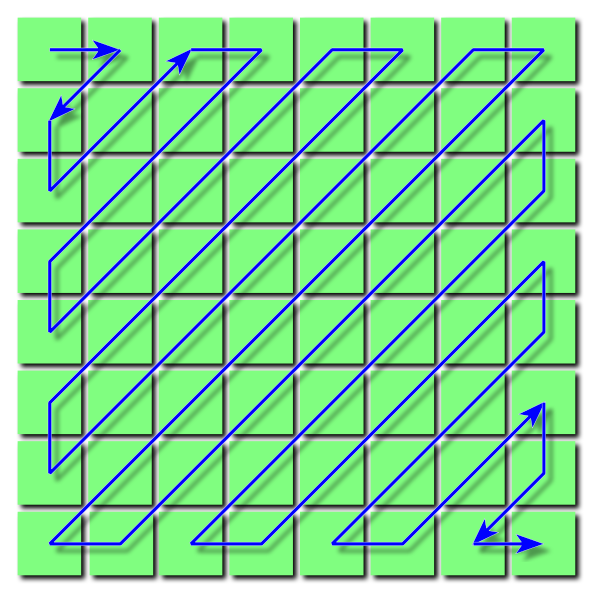
\includegraphics[width=0.5\textwidth]{images/21.png}
        \caption{Zigzag ordering of JPEG image components.}
    \end{figure}
    The previous quantized DC coefficient is used to predict the current quantized DC coefficient. The difference between the two is encoded rather than the actual value. The encoding of the 63 quantized AC coefficients does not use such prediction differencing.
\end{itemize}
\begin{figure}[H]
    \centering
    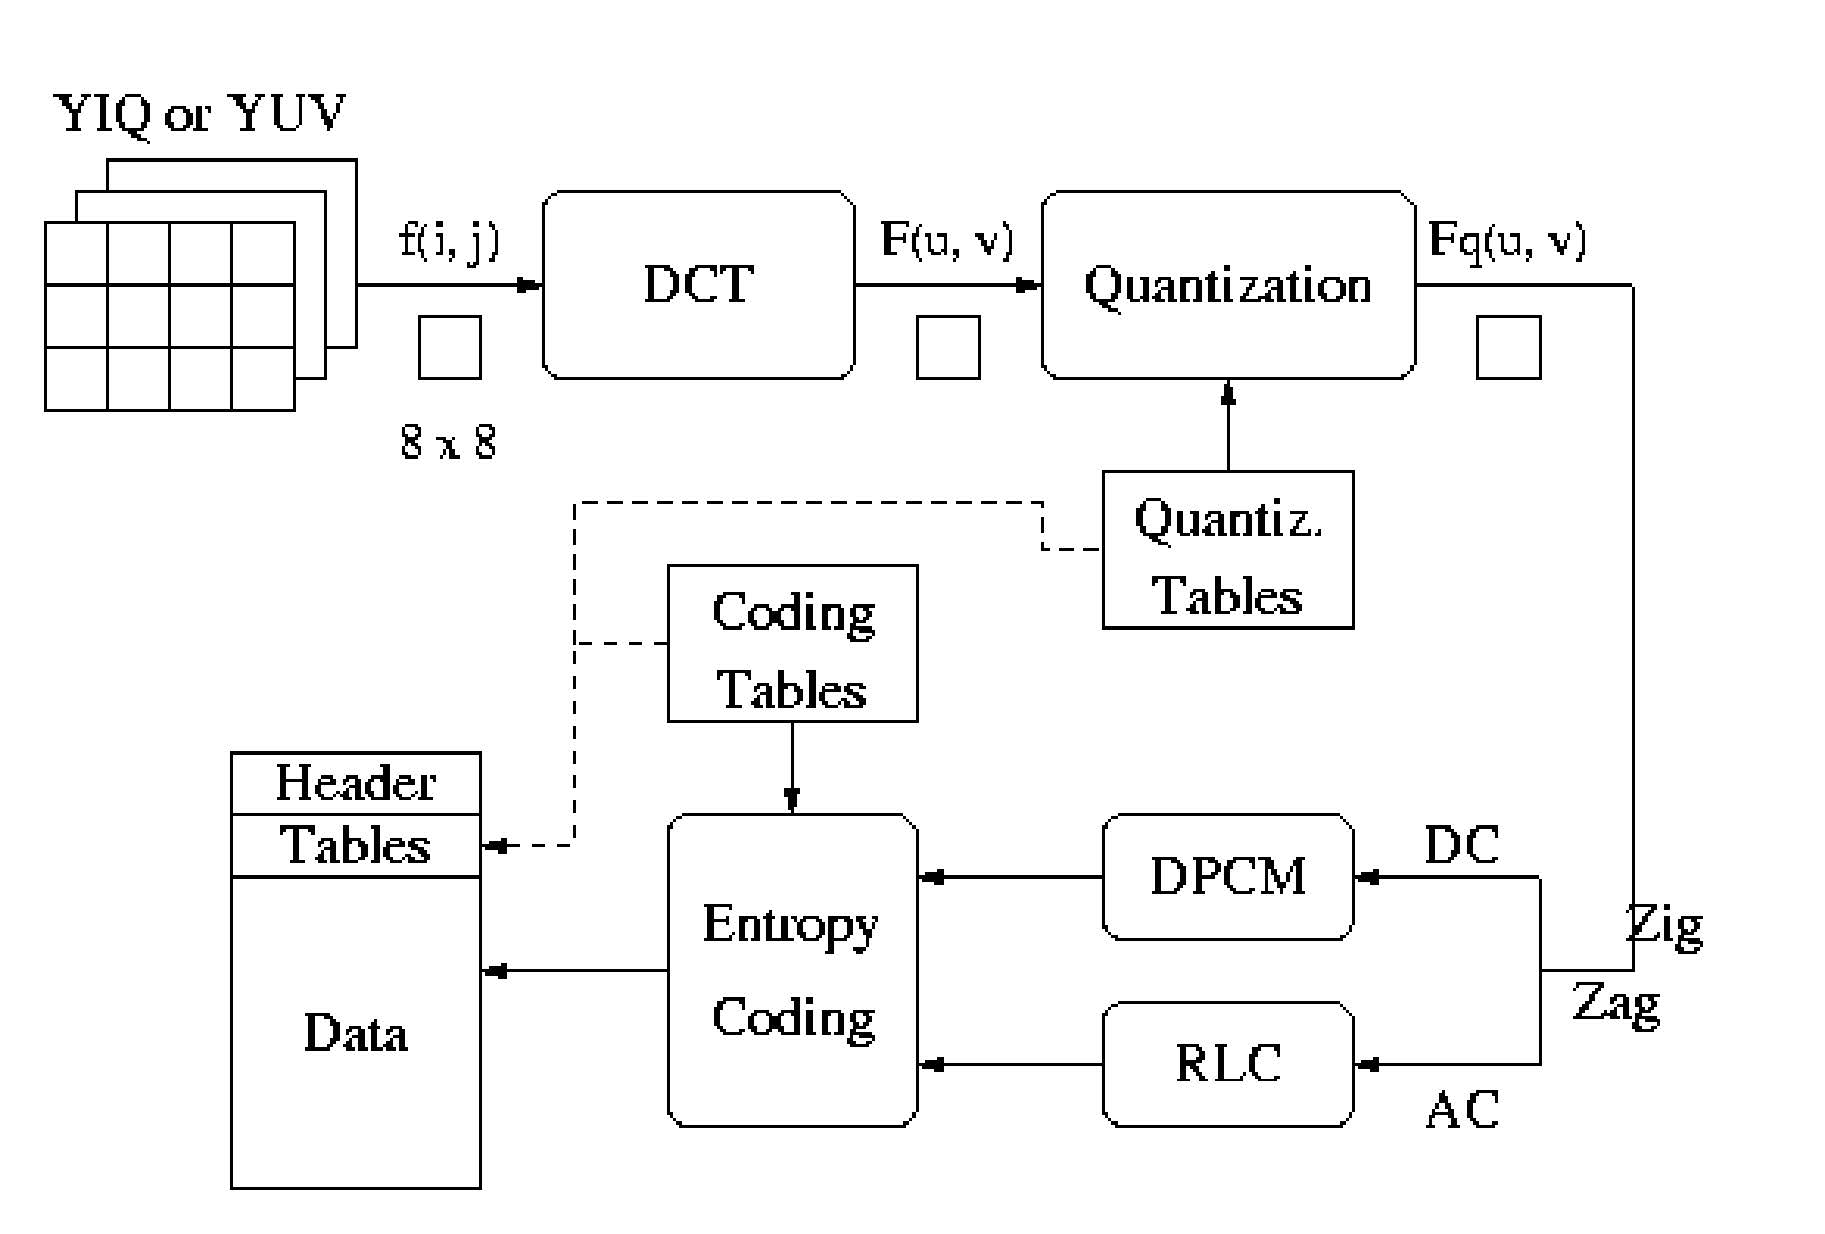
\includegraphics[width=0.8\textwidth]{images/23.jpg}
    \caption{JPEG encoding overview \cite{compression}.}
\end{figure}
The decoding is basically just reversing the three steps. There are two popular implementations of the JPEG standard: \href{https://github.com/LuaDist/libjpeg}{libjpeg} in C and \href{https://github.com/libjpeg-turbo/libjpeg-turbo}{libjpeg-turbo} in C and assembly. For example, you can see how they implement integer DCT and IDCT in libjpeg/jfdctint.c and libjpeg/jidctint.c, and you will see how are macros like \texttt{CONST\_BITS} and \texttt{DESCALE} defined. JPEG or MPEG standards did not exactly specify  which IDCT was to be used by decoders or which coding to be used for compression.

It is exciting that you have already done 2/3 of the work of JPEG encoding. However, the last part is not very simple. If you are familiar with video encoding algorithms, you will find that the three steps can also be seen in the encoding of video formats like H.264/AVC or HEVC. You may choose to complete a simple JPEG encoder/decoder or a simple video encoder/decoder in your final project.
\subsection{Butterfly algorithm}
Previously, you may notice that libjpeg implements DCT and IDCT in different ways. This is because it uses an algorithm called the butterfly algorithm, which is also used in structured linear maps like the discrete Fourier transform (DFT), discrete sine transform (DST), etc \cite{butterfly}. It is not simple to implement the entropy coding now, but you can optionally implement the butterfly algorithm for your DCT.

A good integer DCT has the following requirements:
\begin{itemize}
    \item Bit-exact implementation strictly required.
    \item Must be separable, i.e. the 2D DCT factors into 1D DCT steps.
    \item Must be a close approximation to the DCT.
    \item Basis vectors must be fully orthogonal (or very close).
\end{itemize}

Before exploiting the algorithm, you should learn a diagram called the butterfly diagram. In the context of fast Fourier transform algorithms, a butterfly is a portion of the computation that combines the results of smaller discrete Fourier transforms (DFTs) into a larger DFT, or vice versa (breaking a larger DFT up into sub-transforms). Generally, A butterfly is the transform $(a, b) \mapsto (a + b, a - b)$. A butterfly is also its own inverse, up to a scale factor of two, since $(a+b) + (a-b) = 2a$ and likewise $(a+b) - (a-b) = 2b$ \cite{ryg}. The name "butterfly" comes from the shape of the data-flow diagram in the radix-2 case.
\begin{equation}
    y_{0}=x_{0}+x_{1}
\end{equation}
\begin{equation}
    y_{1}=x_{0}-x_{1}
\end{equation}
If one draws the data-flow diagram for this pair of operations, the (x0, x1) to (y0, y1) lines cross and resemble the wings of a butterfly, hence the name \cite{enwiki:1111230153}.
\begin{figure}[H]
    \centering
    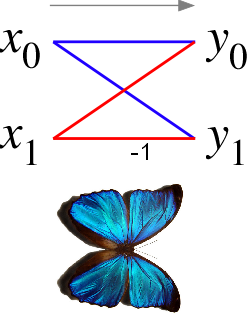
\includegraphics[width=0.6\textwidth]{images/22.png}
    \caption{Signal-flow graph connecting the inputs x (left) to the outputs y that depend on them (right) for a "butterfly" step. This diagram resembles a butterfly (as in the morpho butterfly shown for comparison), hence the name, although in some countries it is also called the hourglass diagram \cite{butterflypic}.}
\end{figure}
Consider the $4\times4$ DCT basis matrix:
\begin{equation}
    \mathbf{A}=\begin{pmatrix}
        \frac{1}{\sqrt{2}}&\frac{1}{\sqrt{2}}&\frac{1}{\sqrt{2}}&\frac{1}{\sqrt{2}}\\
        \frac{\cos{\left(\frac{\pi}{8}\right)}}{\sqrt{2}}&\frac{\sin{\left(\frac{\pi}{8}\right)}}{\sqrt{2}}&-\frac{\sin{\left(\frac{\pi}{8}\right)}}{\sqrt{2}}&-\frac{\cos{\left(\frac{\pi}{8}\right)}}{\sqrt{2}}\\
        \frac{1}{2}&-\frac{1}{2}&-\frac{1}{2}&\frac{1}{2}\\
        \frac{\sin{\left(\frac{\pi}{8}\right)}}{\sqrt{2}}&-\frac{\cos{\left(\frac{\pi}{8}\right)}}{\sqrt{2}}&\frac{cos{\left(\frac{\pi}{8}\right)}}{\sqrt{2}}&-\frac{\sin{\left(\frac{\pi}{8}\right)}}{\sqrt{2}}
    \end{pmatrix}
\end{equation}
Let
\begin{equation}
    \begin{array}{ll}
    a&=\frac{1}{\sqrt{2}}\\
    b&=\frac{\cos{\left(\frac{\pi}{8}\right)}}{\sqrt{2}}\\
    c&=\frac{\sin{\left(\frac{\pi}{8}\right)}}{\sqrt{2}}
    \end{array}
\end{equation}
Then
\begin{equation}
    \mathbf{A}=\begin{pmatrix}
        a&a&a&a\\
        b&c&-c&b\\
        a&-a&-a&a\\
        c&-b&b&-c
    \end{pmatrix}
\end{equation}
Remember the DCT and IDCT are calculated by
\begin{equation}\label{dctbasiseq}
    \mathbf{Y}=\mathbf{AXA}^T
\end{equation}
\begin{equation}
    \mathbf{X}=\mathbf{A}^T\mathbf{YA}
\end{equation}
respectively, where $\mathbf{X}$ is the original image. Then, Equation \ref{dctbasiseq} is equivalent to
\begin{equation}
    \mathbf{Y}=(\mathbf{CXC}^T)\cdot\mathbf{E}=\left(\begin{bmatrix}
        1&1&1&1\\
        1&d&-d&-1\\
        1&-1&-1&1\\
        d&-1&1&-d
    \end{bmatrix}\mathbf{X}\begin{bmatrix}
        1&1&1&d\\
        1&d&-1&-1\\
        1&-d&-1&1\\
        1&-1&1&-d
    \end{bmatrix}
    \right)\cdot\begin{bmatrix}
        a^2&ab&a^2&ab\\
        ab&b^2&ab&b^2\\
        a^2&ab&a^2&ab\\
        ab&b^2&ab&b^2
    \end{bmatrix}
\end{equation}
where $d=\frac{c}{b}=\tan{\frac{\pi}{8}}=\sqrt{2}-1$, $\cdot$ is the element-wise matrix multiplication. To simplify, take $d=0.5$. To keep the orthogonality of the transform, modify $b=\sqrt{\frac{2}{5}}$. Multiply the second and the fourth row of $\mathbf{C}$ and modify $\mathbf{E}$:
\begin{equation}
    \mathbf{Y}=(\mathbf{C}_f\mathbf{XC}_f^T)\cdot\mathbf{E}_f=\left(\begin{bmatrix}
        1&1&1&1\\
        2&1&-1&-2\\
        1&-1&-1&1\\
        1&-2&2&-1
    \end{bmatrix}\mathbf{X}\begin{bmatrix}
        1&2&1&1\\
        1&1&-1&-2\\
        1&-1&-1&2\\
        1&-2&1&-1
    \end{bmatrix}
    \right)\cdot\begin{bmatrix}
        a^2&\frac{ab}{2}&a^2&\frac{ab}{2}\\
        \frac{ab}{2}&\frac{b^2}{4}&\frac{ab}{2}&\frac{b^2}{4}\\
        a^2&\frac{ab}{2}&a^2&\frac{ab}{2}\\
        \frac{ab}{2}&\frac{b^2}{4}&\frac{ab}{2}&\frac{b^2}{4}
    \end{bmatrix}
\end{equation}
The element-wise matrix multiplication ($\cdot\mathbf{E}_f$) do multiplication on each matrix element only once and will be reduced to the quantization process. Thus, the equation only contains integer addition, subtraction, and shifting (multiply by 2) \cite{h264avc}.
\begin{figure}[H]
    \centering
    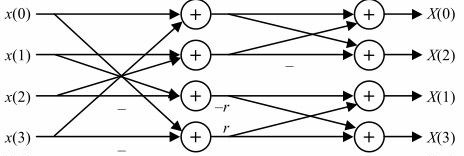
\includegraphics[width=0.6\textwidth]{images/24.jpg}
    \caption{1-D fast transform algorithm ($r=2$ for integer DCT, $r=1$ for Hadamard transform) \cite{h264avc}.}
\end{figure}
Consider one column of $\mathbf{X}$,
\begin{equation}
    \begin{bmatrix}
        1&1&1&1\\
        2&1&-1&-2\\
        1&-1&-1&1\\
        1&-2&2&-1
    \end{bmatrix}\begin{bmatrix}
        x_{01}\\
        x_{11}\\
        x_{21}\\
        x_{31}
    \end{bmatrix}=
    \begin{bmatrix}
        (x_{01}+x_{31})+(x_{11}+x_{21})\\
        2(x_{01}-x_{31})+(x_{11}-x_{21})\\
        (x_{01}+x_{31})-(x_{11}+x_{21})\\
        (x_{01}-x_{31})-2(x_{11}-x_{21})
    \end{bmatrix}
\end{equation}
We found that there are four terms that are to be calculated twice, so can be optimized by the butterfly algorithm. For $8\times8$ DCT, the butterfly diagram is \cite{ryg}
\begin{figure}[H]
    \centering
    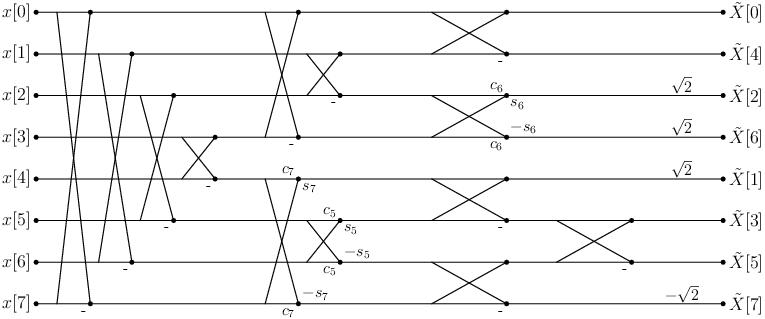
\includegraphics[width=\textwidth]{images/25.png}
\end{figure}
\begin{figure}[H]
    \centering
    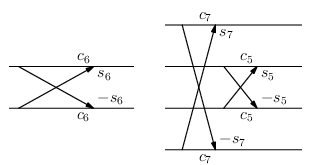
\includegraphics[width=0.6\textwidth]{images/26.png}
\end{figure}
The sample MATLAB provided by \cite{ryg} is
\inputminted[breaklines,linenos]{matlab}{bink_dct_B2.m}
Modify your \texttt{dct.c} and verify the correctness of your results. Generate the output data file \texttt{output.dat}. Create a new Vitis HLS solution with butterfly DCT and compare it with the previous DCT by Vitis HLS Report Comparison.

\section{Introduction to PYNQ Overlays}\label{SPynq}
\subsection{Load a PYNQ overlay}\label{S51}
Overlays, or hardware libraries, are programmable/configurable FPGA designs that extend the user application from the Processing System of the Zynq into the Programmable Logic. Overlays can accelerate a software application or customize a hardware platform for a particular application.

For example, image processing is a typical application where the FPGAs can provide acceleration. A software programmer can use an overlay in a similar way to a software library to run some of the image processing functions (e.g. edge detection, thresholding, etc.) on the FPGA fabric. Overlays can be loaded to the FPGA dynamically, as required, just like a software library. In this example, separate image processing functions could be implemented in different overlays and loaded from Python on demand.

PYNQ provides a Python interface to allow overlays in the PL to be controlled from Python running in the PS. FPGA design is a specialized task that requires hardware engineering knowledge and expertise. PYNQ overlays are created by hardware designers and wrapped with this PYNQ Python API. Software developers can then use the Python interface to program and control specialized hardware overlays without needing to design an overlay themselves. This is analogous to software libraries created by expert developers, which are then used by many other software developers working at the application level.

By default, an overlay (bitstream) called base is downloaded into the PL at boot time. The base overlay can be considered a reference design for a board. New overlays can be installed or copied to the board and loaded into the PL as the system runs.

An overlay usually includes:
\begin{itemize}
    \item A bitstream to configure the FPGA fabric
    \item A Vivado design HWH file to determine the available IP
    \item Python API that exposes the IPs as attributes
\end{itemize}
The PYNQ \texttt{Overlay} class can be used to load an overlay. An overlay is instantiated by specifying the name of the bitstream file. Instantiating the Overlay also downloads the bitstream by default and parses the HWH file.

For the base overlay, we can use the existing \texttt{BaseOverlay} class; this class exposes the IPs available on the bitstream as attributes of this class.

Open PYNQ. If the browser shows \verb|DNS_PROBE_FINISHED_NXDOMAIN|, run
\begin{minted}{bat}
ipconfig /flushdns
\end{minted}
Note that the Jupyter notebook home directory is \verb|root@pynq:/home/xilinx/jupyter_notebooks|. You can check by \texttt{ls} command. You can also access the file explorer of Windows by \verb|\\pynq|. However, operating files are directories in Terminal is much faster than file explorer.

Create a new Python 3 notebook.
\begin{minted}{python}
from pynq.overlays.base import BaseOverlay
base_overlay = BaseOverlay("base.bit")
\end{minted}
Once an overlay has been instantiated, the \texttt{help()} method can be used to discover what is in an overlay. The help information can be used to interact with the overlay. Note that if you try the following code on your own board, you may see different results depending on the version of PYNQ you are using, and which board you have.
\begin{minted}{python}
help(base_overlay)
\end{minted}
This will give a list of the IPs and methods available as part of the overlay.

From the \texttt{help()} printout above, it can be seen that in this case, the overlay includes a \texttt{gpio\_dict} instance:
\begin{minted}{python}
"""
leds : AxiGPIO

     4-bit output GPIO for interacting with the green LEDs LD0-3
"""
\end{minted}
Running \texttt{help()} on the \texttt{gpio\_dict} object will provide more information about the object, including details of its API.
\begin{minted}{python}
help(base_overlay.leds)
\end{minted}
The API can be used to control the object. For example, the following cell will turn on LD0 on the board.
\begin{minted}{python}
base_overlay.leds[0].toggle()
\end{minted}
Information about other IPs can be found from the overlay instance in a similar way, as shown below.
\begin{minted}{python}
help(base_overlay.video)
\end{minted}
Save your Jupyter notebook as \texttt{lab3\_1.ipynb} with outputs.
\subsection{Partial configuration}\label{S52}
From image v2.4, PYNQ supports partial bitstream reconfiguration. The partial bitstreams are managed by the overlay class. It is always recommended to use the .hwh file along with the .bit for the overlay class.

\subsubsection{Preparing the files}
There are many ways to prepare bitstreams. Users can choose to follow the project flow or the software flow to implement a partial reconfiguration Vivado project. For more information, please refer to the documentation page on partial reconfiguration.

After each reconfiguration, the PL status will update to reflect the changes on the bitstream, so that new drivers can be assigned to the new blocks available in the bitstream. To achieve this, users have to provide the metadata file (.hwh file) along with each full/partial bitstream. The .hwh file is typically located at: <project\_name>/<design\_name>.gen/\\
sources\_1/bd/<design\_name>/hw\_handoff/.

Keep in mind that each partial bitstream needs a .hwh file.

In this lab, we will use boards/Pynq-Z1/gpio\_pr/notebooks/partial\_reconfig from \url{https://github.com/yunqu/partial_reconfig_example}.
\subsubsection{Loading full bitstream}
It is straightforward to download a full bitstream. By default, the bitstream will be automatically downloaded onto the PL when users instantiate an overlay object.
\begin{minted}{python}
from pynq import Overlay
overlay = Overlay('gpio_pr.bit')
\end{minted}
To download the full bitstream again:
\begin{minted}{python}
overlay.download()
\end{minted}
Note that no argument is provided if a full bitstream is to be downloaded.

Another thing to note, is that if the Vivado project is configured as a partial reconfiguration project, the .hwh file for the full bitstream will not contain any information inside a partial region, even if the full bitstream always has a default Reconfiguration Module (RM) implemented. Instead, the .hwh file only provides information on the interfaces connecting to the partial region. So for the full bitstream, do not be surprised if you see an empty partial region in the .hwh file. The complete information on the partial regions are revealed by the .hwh files of the partial bitstreams, where each .hwh file reveals one possible internal organization of the partial region.

Run
\begin{minted}{python}
from pprint import pprint
pprint(overlay.interrupt_pins)
pprint(overlay.pr_dict)
\end{minted}
\subsubsection{Loading partial bitstream}
Typically, the partial regions are hierarchies in the block design of the bitstream. In an overlay object, the hierarchical blocks are exposed as attributes of the object. In the following example, let us assume there is a hierarchical block called gpio\_0 in the design. There are two ways to download a partial bitstream.

The first way, using the \texttt{download()} method of the \texttt{DefaultHierarchy} class, please see \texttt{pynq.overlay.DefaultHierarchy.download()}.

The second way, using \texttt{pr\_download()} method of the \texttt{Overlay} class. For this, users have to specify the partial region as well as the partial bitstream, see \texttt{pynq.overlay.Overlay.pr\_\\
download()}.
\begin{minted}{python}
overlay.pr_download('gpio_0', 'led_5.bit')
\end{minted}
Observe the LEDs change on your board. Take a photo of your board. To load a different RM:
\begin{minted}{python}
overlay.pr_download('gpio_0', 'led_a.bit')
\end{minted}
Take another photo of your board. Save your Jupyter notebook as \texttt{lab3\_2.ipynb} with outputs.
\subsection{PYNQ HelloWorld}\label{S53}
Open a terminal on your PYNQ board and run:
\begin{minted}{bash}
sudo pip3 install pynq-helloworld --no-build-isolation
\end{minted}
\begin{figure}[H]
    \centering
    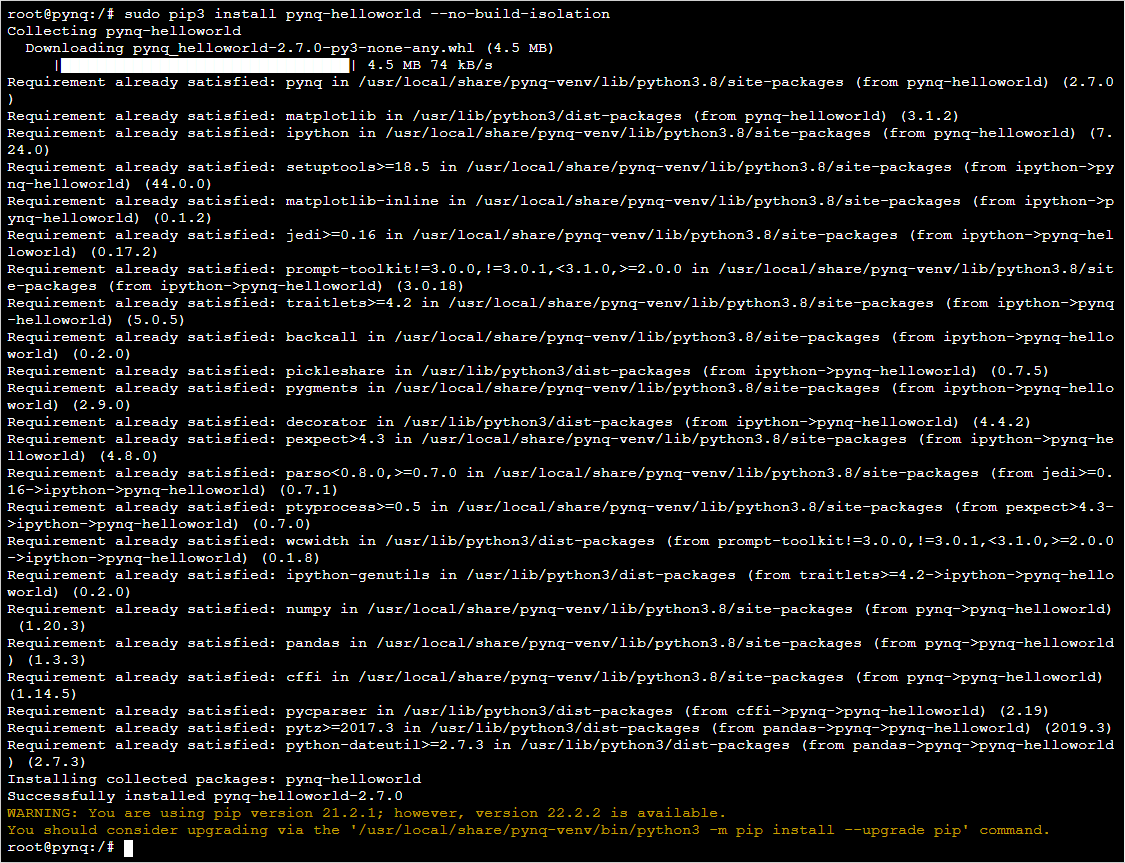
\includegraphics[width=\textwidth]{images/27.png}
\end{figure}
Currently, this repository is compatible with pynq package v2.7.0.

Go to your Jupyter home folder (on our boards, this is /home/xilinx/jupyter\_notebooks), and run the following to deliver the notebooks:
\begin{minted}{bash}
pynq get-notebooks pynq-helloworld -p .
\end{minted}
Run all cells of pynq-helloworld/resizer\_pl.ipynb and pynq-helloworld/resizer\_ps.ipynb. Take screenshots of your outputs. Explain your results.
\subsection{Creating overlays}\label{S54}
Go through the "Developing a Single IP" section and the "Creating a Driver" section in \href{https://pynq.readthedocs.io/en/latest/overlay_design_methodology/overlay_tutorial.html}{Overlay Tutorial}.
% Use any bitstreams we generated in previous labs.
The sample Jupyter notebook is \cite{pynqadder} \cite{csdnoverlay}:
\begin{minted}{python}
from pynq import Overlay

overlay = Overlay('../pynq_adder.bit')
overlay?
add_ip = overlay.scalar_add
add_ip?
add_ip.register_map
add_ip.register_map.a = 3
add_ip.register_map.b = 4
add_ip.register_map.c
add_ip.write(0x10, 4)
add_ip.write(0x18, 5)
add_ip.read(0x20)
from pynq import DefaultIP

class AddDriver(DefaultIP):
    def __init__(self, description):
        super().__init__(description=description)

    bindto = ['xilinx.com:hls:hls_adder:1.0']

    def add(self, a, b):
        self.write(0x10, a)
        self.write(0x18, b)
        return self.read(0x20)
overlay = Overlay('../pynq_adder.bit')
overlay?
overlay.scalar_add.add(15,20)
\end{minted}
Save your Jupyter notebook as \texttt{lab3\_3.ipynb} with outputs.
\subsection{Questions}\label{S5Q}
\begin{enumerate}
    \item Please list out any advantages of using overlay.
    \item In general, when you choose the software approach vs. hardware acceleration approach, what are the considerations? Any tradeoffs?
\end{enumerate}

% \section{Introduction to FINN}
% FINN is an experimental framework from Xilinx Research Labs to explore deep neural network inference on FPGAs. It specifically targets quantized neural networks (QNNs), with an emphasis on generating dataflow-style architectures customized for each network. It is not intended to be a generic DNN accelerator offering like Vitis AI, but rather a tool for exploring the design space of DNN inference accelerators on FPGAs.
% \section{(Optional) Use PYNQ overlay to verify the correctness of your DCT}
\section{(Optional) FIR Filter on PYNQ}\label{Sopt2}
\subsection{Implementation and optimization of an FIR filter by HLS}
According to Lab 3 slides, implement a functionally correct, but not optimized, 128-tap FIR filter. This is your baseline implementation. Use the provided script.tcl to create your project. Try the following optimization:
\begin{itemize}
    \item Variable Bitwidths: It is possible to specify a very precise data type for each variable in your design. The number of different data types is extensive: floating point, integer, and fixed point, all with varying bit widths and options. The data type provides a tradeoff between accuracy, resource usage, and performance.
    \item Pipelining: Pipelining increases the throughput typically at the cost of additional resources. The initiation interval (II) is an important design parameter that changes performance and resource usage.
    \item Removing Conditional Statements: If/else statements and other conditionals can limit the possible parallelism and often require additional resources. If the code can be rewritten to remove them, it can make the resulting design more efficient. This is known as code hoisting.
    \item Loop Partitioning: Dividing the loop into two or more separate loops may allow for each of those loops to be executed in parallel (via unrolling), enable loop level pipelining, or provide other benefits. This may increase performance and resource usage.
    \item Memory Partitioning: The storage of the arrays in memory plays an important role in area and performance. On the one hand, you could put an array entirely in one memory (e.g., BRAM). But this limits the number of read accesses and write accesses per cycle. Or you can divide the array into two or more memories to increase the number of ports. Or you could instantiate each of the variables as its own register, which allows simultaneous access to all of the variables at every clock cycle.
\end{itemize}
Combine any number of optimizations to get your best architecture. A design with high throughput will likely take a lot of resources. A design that has small resource usage likely will have lower performance, but that could still be the best depending on the application goals. It is possible that some optimizations may not have a big (or any effect). Some optimizations may only work when you use them in combination with others. This is what makes the design space exploration process difficult.
\subsection{From HLS to PYNQ}
\begin{enumerate}
    \item HLS to RTL: Run C Synthesis, Implementation, and export RTL in Vitis HLS. \textit{Sometimes you may need to set port types before synthesis: Make sure that fir\_test.cpp is open. Open Directive and right click on the options, and select Modify Directive. In the drop-down, select INTERFACE and set all the ports to s\_axilite by right-clicking on available options. Repeat the same for all the options.}
    \item RTL to Bitstream: Add FIR Filter IP to your block design in your Vivado project with ZYNQ7 Processing System. Generate bitstream. Before closing Vivado, we need to note our IP and its port addresses. Under Sources, open fir\_test\_fir\_io\_s\_axi.v, scroll down and note addresses for in and out ports. We need these addresses for our host program. For example, the addresses to pay attention to are 0x00 (control bus ap\_ctrl), 0x10 (output), and 0x18 (input). These are the addresses you will need to use to write data to the fabric from the ARM core, start the fabric to run your design and generate your outputs, and then read your outputs from the fabric into the ARM core on the Pynq board.
    \item Bitstream on PYNQ: Make sure to name the .bit file and the .hwh file with the same name. For example, we name them “design\_1\_wrapper.bit” and “design\_1\_wrapper.hwh”.
\end{enumerate}
\subsection{Verification on PYNQ}
Write a host program host\_fir.ipynb. The example usage of MMIO is
\begin{minted}[breaklines,linenos]{python}
from pynq import Overlay
from pynq import MMIO
ol = Overlay("/home/xilinx/jupyter_notebooks/fir_test/design_1_wrapper.bit") # designate a bitstream to be flashed to the FPGA
ol.download() # flash the FPGA
fir_ip = MMIO(0x43C00000, 0x10000) # (IP_BASE_ADDRESS, ADDRESS_RANGE), told to us in Vivado
inp = 5
fir_ip.write(0x18, inp) # write input value to input address in fabric
print("input:", fir_ip.read(0x18)) # confirm that our value was written correctly to the fabric
fir_ip.write(0x00, 1) # set ap_start to 1 which initiates the process we wrote to the fabric
print("output:", fir_ip.read(0x10)) # read corresponding output value from the output address of the fabric
\end{minted}
Use \texttt{matplotlib} to plot the input data vs. time and the output data vs. time. The sample image by the 11-tap FIR filter is as shown below:
\begin{figure}[H]
    \centering
    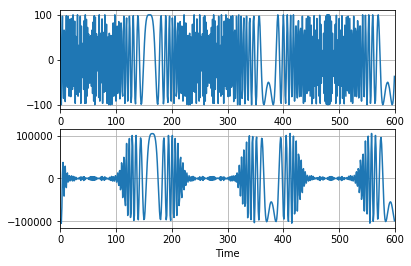
\includegraphics[width=\textwidth]{images/28.png}
\end{figure}
You are expected to show a similar image using the output of your 128-tap FIR filter.

\newpage
\section{Deliverables}
% You only need to choose one from Section \ref{Sopt1} and \ref{Sopt2}.
\begin{enumerate}
    \item Section \ref{S2}:
    \begin{enumerate}
        \item Section \ref{S23}: answer the questions
        \item Section \ref{S24}: the screenshot of the Performance Estimates and Utilization Estimates of the Vitis HLS Report Comparison.
        \item Section \ref{S25}: the screenshot of the Performance Estimates and Utilization Estimates of the Synthesis Details Report after \texttt{DATAFLOW} directive is applied
        \item Section \ref{S25}: the screenshot of the Performance Estimates and Utilization Estimates of the Synthesis Details Report after configuring Dataflow commands
        \item Section \ref{S26} (Optional): the screenshot of your implementation report and the exported RTL zip file
    \end{enumerate}
    \item Section \ref{S3}:
    \begin{enumerate}
        \item Section \ref{S34}: answer the questions in Step 4
        \item Section \ref{S35}: the screenshot of the Utilization Estimates detail of memory in Step 5
        \item Section \ref{S37}: the screenshot of the Performance Estimates and the Utilization Estimates of the Vitis HLS Report Comparison between all five solutions
        \item Section \ref{S3idct}: the modified \texttt{dct.c} code and the generated output data file \texttt{output.dat}
        \item Section \ref{S3idct} (Optional): the recovered image
    \end{enumerate}
    \item Section \ref{Sopt1} (Optional): the modified \texttt{dct.c} code, \texttt{output.dat}, and the report comparison (if you finish this section, no need to finish Section \ref{Sopt2})
    \item Section \ref{SPynq}:
    \begin{enumerate}
        \item Section \ref{S51}: the lab3\_1.ipynb code with outputs
        \item Section \ref{S52}: the two photos of the board and the lab3\_2.ipynb code with outputs
        \item Section \ref{S53}: the screenshots of the outputs of resizer\_pl.ipynb and the outputs of resizer\_ps.ipynb
        \item Section \ref{S54}: the lab3\_3.ipynb code with outputs
        \item Section \ref{S5Q}: answer to the questions
    \end{enumerate}
    \item Section \ref{Sopt2} (Optional): the \texttt{fir.cpp} code and the \texttt{host\_fir.ipynb} including the plots (if you finish this section, no need to finish Section \ref{Sopt1})
\end{enumerate}
\section{Grading policy}
% \textbf{If you want to }
\begin{table}[H]
    \centering
    \begin{tabular}{|c|c|}
        \hline
        Factors & Percentage \\
        \hline
        Section \ref{S2} & 35\% + 2\% bonus \\
        \hline
        Section \ref{S3} & 35\% + 3\% bonus \\
        \hline
        Section \ref{Sopt1} & 20\% bonus (not take effect concurrently with Section \ref{Sopt2}) \\
        \hline
        Section \ref{SPynq} & 30\% \\
        \hline
        Section \ref{Sopt2} & 20\% bonus (not take effect concurrently with Section \ref{Sopt1}) \\
        \hline
    \end{tabular}
\end{table}

\newpage
\appendix
\section{Peer Evaluation Form}
\begin{table}[H]
    \centering
    \begin{tabular}{|c|c|c|c|c|}
        \hline
        Part & Your work & Your partner's work & Your score & Your partner's score \\
        \hline
        Section \ref{S2} & & & & \\
        \hline
        Section \ref{S3} & & & & \\
        \hline
        Section \ref{Sopt1} & & & & \\
        \hline
        Section \ref{SPynq} & & & & \\
        \hline
        Section \ref{Sopt2} & & & & \\
        \hline
    \end{tabular}
\end{table}

\newpage
\section{Troubleshooting}
\subsection{Vitis HLS Command Prompt Make}\label{AMake}
If you failed to run \texttt{make} in Vitis, read \cite{make}. This is an old bug since at least Vitis HLS 2021.1. It was reported by Prof. Guo and me last year, but it is still not fixed, as Xilinx always does not care about thousands of user-reported bugs on its support website, especially for those on the Windows platform. Generally, your system PATH does not contain \texttt{gcc}, so just change Line 3 of \texttt{vitis\_hls\_cmd.bat} to
\begin{minted}[breaklines,breakanywhere,linenos,escapeinside=||]{bat}
set PATH=%~dp0;%PATH%;%~dp0..\tps\win64\msys64\usr\bin;%~dp0..\tps\win64\msys64\mingw64\bin|\setcounter{FancyVerbLine}{3}|
\end{minted}
After doing that, you may also change Line 6 to:
\begin{minted}[breaklines,linenos,escapeinside=||]{bat}
set VITIS_HLS_HOME=%~dp0..|\setcounter{FancyVerbLine}{6}|
\end{minted}
\subsection{Vitis HLS FIFO Configuration}\label{AFifo}
This is an old bug since at least Vitis HLS 2021.1. It was reported by Prof. Guo and me last year, but it is still not fixed. In viis\_hls.log, you can see:
\begin{minted}[breaklines,breakanywhere]{text}
INFO: [RTMG 210-285] Implementing FIFO 'Y_scale_c_U(yuv_filter_fifo_w8_d3_S)' using Shift Registers.
INFO: [RTMG 210-285] Implementing FIFO 'U_scale_c_U(yuv_filter_fifo_w8_d3_S)' using Shift Registers.
INFO: [RTMG 210-285] Implementing FIFO 'V_scale_c_U(yuv_filter_fifo_w8_d3_S)' using Shift Registers.
INFO: [RTMG 210-285] Implementing FIFO 'p_yuv_channels_ch1_U(yuv_filter_fifo_w8_d2457600_A)' using Vivado Default RAMs.
INFO: [RTMG 210-285] Implementing FIFO 'p_yuv_channels_ch2_U(yuv_filter_fifo_w8_d2457600_A)' using Vivado Default RAMs.
INFO: [RTMG 210-285] Implementing FIFO 'p_yuv_channels_ch3_U(yuv_filter_fifo_w8_d2457600_A)' using Vivado Default RAMs.
INFO: [RTMG 210-285] Implementing FIFO 'p_yuv_width_U(yuv_filter_fifo_w16_d2_S)' using Shift Registers.
INFO: [RTMG 210-285] Implementing FIFO 'p_yuv_height_U(yuv_filter_fifo_w16_d2_S)' using Shift Registers.
INFO: [RTMG 210-285] Implementing FIFO 'p_scale_channels_ch1_U(yuv_filter_fifo_w8_d2457600_A)' using Vivado Default RAMs.
INFO: [RTMG 210-285] Implementing FIFO 'p_scale_channels_ch2_U(yuv_filter_fifo_w8_d2457600_A)' using Vivado Default RAMs.
INFO: [RTMG 210-285] Implementing FIFO 'p_scale_channels_ch3_U(yuv_filter_fifo_w8_d2457600_A)' using Vivado Default RAMs.
INFO: [RTMG 210-285] Implementing FIFO 'p_scale_width_U(yuv_filter_fifo_w16_d2_S)' using Shift Registers.
INFO: [RTMG 210-285] Implementing FIFO 'p_scale_height_U(yuv_filter_fifo_w16_d2_S)' using Shift Registers.
INFO: [RTMG 210-285] Implementing FIFO 'start_for_yuv_scale_U0_U(yuv_filter_start_for_yuv_scale_U0)' using Shift Registers.
INFO: [RTMG 210-285] Implementing FIFO 'start_for_yuv2rgb_1_U0_U(yuv_filter_start_for_yuv2rgb_1_U0)' using Shift Registers.
\end{minted}
The channels are still using Vivado Default RAMs instead of Shift Registers.

Solution 1. Modify Line 10 of your yuv\_filter.prj/solution3/solution3.aps from
\begin{minted}[breaklines,breakanywhere]{text}
> <config_dataflow default_channel="fifo" scalar_fifo_depth="0" start_fifo_depth="0"/>
\end{minted}
to
\begin{minted}[breaklines,breakanywhere]{text}
> <config_dataflow default_channel="fifo" fifo_depth="2" scalar_fifo_depth="0" start_fifo_depth="0"/>
\end{minted}
and redo C Synthesis.

Solution 2. Solution Settings (solution3)->General->Configuration Settings->Commands->config\_storage->fifo impl, change value from default `autosrl` to `srl` and redo C Synthesis.
\begin{figure}[H]
    \centering
    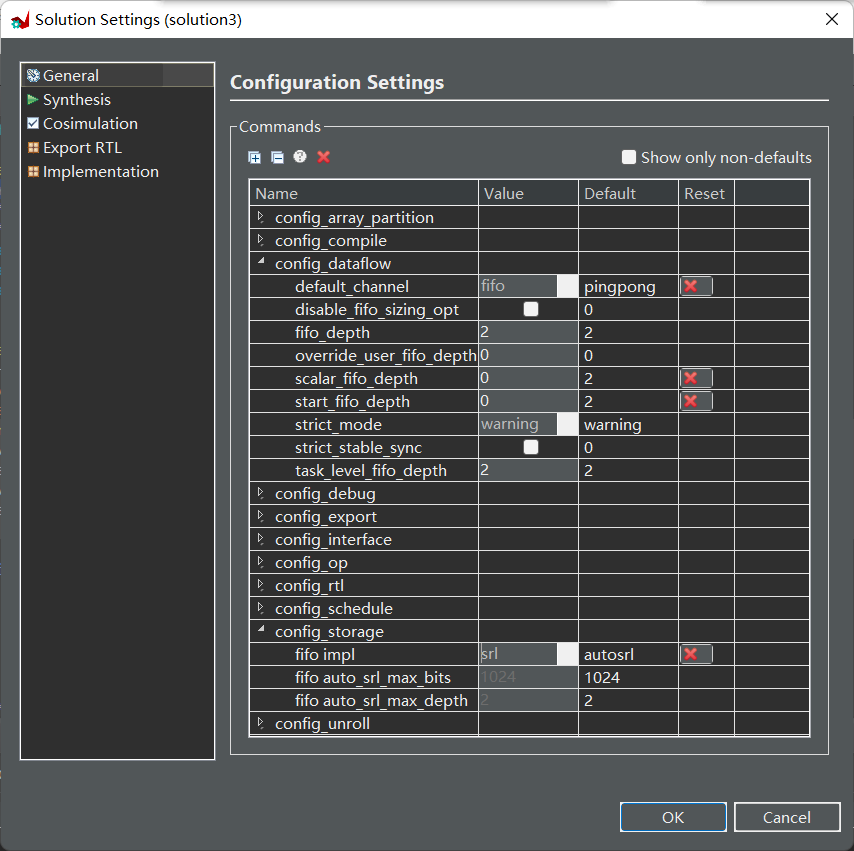
\includegraphics[width=\textwidth]{images/8.png}
\end{figure}

After that, you should see the following information in vitis\_hls.log:
\begin{minted}[breaklines,breakanywhere]{text}
INFO: [RTMG 210-285] Implementing FIFO 'Y_scale_c_U(yuv_filter_fifo_w8_d3_S)' using Shift Registers.
INFO: [RTMG 210-285] Implementing FIFO 'U_scale_c_U(yuv_filter_fifo_w8_d3_S)' using Shift Registers.
INFO: [RTMG 210-285] Implementing FIFO 'V_scale_c_U(yuv_filter_fifo_w8_d3_S)' using Shift Registers.
INFO: [RTMG 210-285] Implementing FIFO 'p_yuv_channels_ch1_U(yuv_filter_fifo_w8_d2457600_S)' using Shift Registers.
INFO: [RTMG 210-285] Implementing FIFO 'p_yuv_channels_ch2_U(yuv_filter_fifo_w8_d2457600_S)' using Shift Registers.
INFO: [RTMG 210-285] Implementing FIFO 'p_yuv_channels_ch3_U(yuv_filter_fifo_w8_d2457600_S)' using Shift Registers.
INFO: [RTMG 210-285] Implementing FIFO 'p_yuv_width_U(yuv_filter_fifo_w16_d2_S)' using Shift Registers.
INFO: [RTMG 210-285] Implementing FIFO 'p_yuv_height_U(yuv_filter_fifo_w16_d2_S)' using Shift Registers.
INFO: [RTMG 210-285] Implementing FIFO 'p_scale_channels_ch1_U(yuv_filter_fifo_w8_d2457600_S)' using Shift Registers.
INFO: [RTMG 210-285] Implementing FIFO 'p_scale_channels_ch2_U(yuv_filter_fifo_w8_d2457600_S)' using Shift Registers.
INFO: [RTMG 210-285] Implementing FIFO 'p_scale_channels_ch3_U(yuv_filter_fifo_w8_d2457600_S)' using Shift Registers.
INFO: [RTMG 210-285] Implementing FIFO 'p_scale_width_U(yuv_filter_fifo_w16_d2_S)' using Shift Registers.
INFO: [RTMG 210-285] Implementing FIFO 'p_scale_height_U(yuv_filter_fifo_w16_d2_S)' using Shift Registers.
INFO: [RTMG 210-285] Implementing FIFO 'start_for_yuv_scale_U0_U(yuv_filter_start_for_yuv_scale_U0)' using Shift Registers.
INFO: [RTMG 210-285] Implementing FIFO 'start_for_yuv2rgb_1_U0_U(yuv_filter_start_for_yuv2rgb_1_U0)' using Shift Registers.
\end{minted}
\subsection{Vitis HLS Export RTL ERROR IMPL}\label{AImpl}
Check yuv\_filter.prj/solution3/impl/ip/hs\_err\_pid38996.log, reboot your computer, and re-run implementation. You can specify IP Location, and it will automatically export RTL there.

\section{Change Log}
Fall 2022: Yihua Liu
\begin{itemize}
    \item merged Lab 3 and Lab 4 from Word to LaTeX
    \item added an introduction to YUV model and updated the starter code
    \item updated Section \ref{SPynq}
    \item added Section \ref{S3}, \ref{Sopt1}, \ref{Sopt2}, and the troubleshooting section
\end{itemize}
Fall 2021: Prof. Xinfei Guo
\begin{itemize}
    \item created this lab of optimizing performance through pipelining as Lab 4
    \item created this lab of PYNQ overlays as Lab 3
\end{itemize}

\printbibliography
\end{document}

